% Template KLTN cho SV trường ĐHKHTN
% Liên hệ: nqminh@fit.hcmus.edu.vn
% Last update: 08/06/2016

% Chú ý: đọc các phần chú ý đóng khung của file này và chỉnh lại cho phù hợp.
% Trước khi build, xóa hết các file được tạo ra trong quá trình build trước đó, và build theo thứ tự: BIB > PDF > PDF.
% Nếu cập nhật tài liệu tham khảo, cũng cần build lại theo cách trên.

\documentclass[oneside,a4paper,14pt]{extreport}

% Font tiếng Việt
\usepackage[T5]{fontenc}
\usepackage[utf8]{inputenc}
\DeclareTextSymbolDefault{\DH}{T1}

% Tài liệu tham khảo
\usepackage[
	sorting=nty,
	backend=bibtex,
  maxnames = 5,
	defernumbers=true]{biblatex}
\usepackage[unicode]{hyperref} % Bookmark tiếng Việt
\addbibresource{References/references.bib}

\makeatletter
\def\blx@maxline{77}
\makeatother

% Chèn hình, các hình trong luận văn được để trong thư mục Images/
\usepackage{graphicx}
\graphicspath{ {Images/} }

% Chèn và định dạng mã nguồn
\usepackage{listings}
\usepackage{color}
\definecolor{codegreen}{rgb}{0,0.6,0}
\definecolor{codegray}{rgb}{0.5,0.5,0.5}
\definecolor{codepurple}{rgb}{0.58,0,0.82}
\definecolor{backcolour}{rgb}{0.95,0.95,0.92}
\lstdefinestyle{mystyle}{
    backgroundcolor=\color{backcolour},   
    commentstyle=\color{codegreen},
    keywordstyle=\color{magenta},
    numberstyle=\tiny\color{codegray},
    stringstyle=\color{codepurple},
    basicstyle=\footnotesize,
    breakatwhitespace=false,         
    breaklines=true,                 
    captionpos=b,                    
    keepspaces=true,                 
    numbers=left,                    
    numbersep=5pt,                  
    showspaces=false,                
    showstringspaces=false,
    showtabs=false,                  
    tabsize=2
}
\lstset{style=mystyle}

% Chèn và định dạng mã giả
\usepackage{amsmath}
\usepackage{amsfonts}
\usepackage{algorithm}
\usepackage[noend]{algpseudocode}
\makeatletter
\def\BState{\State\hskip-\ALG@thistlm}
\makeatother
\hypersetup{pdfborder=0 0 0}
% Bảng biểu
\usepackage{multirow}
\usepackage{array}
\newcolumntype{L}[1]{>{\raggedright\let\newline\\\arraybackslash\hspace{0pt}}m{#1}}
\newcolumntype{C}[1]{>{\centering\let\newline\\\arraybackslash\hspace{0pt}}m{#1}}
\newcolumntype{R}[1]{>{\raggedleft\let\newline\\\arraybackslash\hspace{0pt}}m{#1}}

% Đổi tên mặc định
\renewcommand{\chaptername}{Chương}
\renewcommand{\figurename}{Hình}
\renewcommand{\tablename}{Bảng}
\renewcommand{\contentsname}{Mục lục}
\renewcommand{\listfigurename}{Danh sách hình}
\renewcommand{\listtablename}{Danh sách bảng}
\renewcommand{\appendixname}{Phụ lục}

% Dãn dòng 1.5
\usepackage{setspace}
\onehalfspacing

% Thụt vào đầu dòng
\usepackage{indentfirst}

% Canh lề
\usepackage[
  top=30mm,
  bottom=25mm,
  left=30mm,
  right=20mm,
  includefoot]{geometry}
  
% Trang bìa
\usepackage{tikz}
\usetikzlibrary{calc}
\newcommand\HRule{\rule{\textwidth}{1pt}}

% ========================================================================================= %
% CHÚ Ý: Thông tin chung về KLTN - sinh viên điền vào đây để tự động update các trang khác  %
% ========================================================================================= %
\newcommand{\tenSV}{Đào~Đức~Anh~-~Nguyễn~Thành~Nhân} % Dấu ~ là khoảng trắng không được tách (các chữ nối với nhau bằng dấu ~ sẽ nằm cùng 1 dòng
\newcommand{\mssv}{1234567}
\newcommand{\tenKL}{Xây~dựng~hệ~thống~gợi~ý~sản~phẩm~dựa~trên~mô~hình~Auto-Encoder} % Chú ý dấu ~ trong tên khóa luận
\newcommand{\tenGVHD}{Trần~Trung~Kiên}
\newcommand{\tenBM}{Khoa học máy tính}
% \setcounter{tocdepth}{4}
\begin{document}

\begin{titlepage}

\begin{center}
%ĐẠI HỌC QUỐC GIA THÀNH PHỐ HỒ CHÍ MINH\\
TRƯỜNG ĐẠI HỌC KHOA HỌC TỰ NHIÊN\\
\textbf{KHOA CÔNG NGHỆ THÔNG TIN}\\[2cm]


{ \Large \bfseries Đào Đức Anh - Nguyễn Thành Nhân\\[2cm] } 

%Tên đề tài Khóa luận tốt nghiệp/Đồ án tốt nghiệp

{ \Large \bfseries  Xây dựng hệ thống gợi ý sản phẩm\\dựa trên mô hình Auto-Encoder \\[3cm]} 


%Chọn trong các dòng sau
\large KHÓA LUẬN TỐT NGHIỆP CỬ NHÂN\\
%\large ĐỒ ÁN TỐT NGHIỆP CỬ NHÂN\\
%\large THỰC TẬP TỐT NGHIỆP CỬ NHÂN\\
%Đưa vào dòng này nếu thuộc chương trình Chất lượng cao, hoặc lớp Cử nhân tài năng
\large CHƯƠNG TRÌNH CHÍNH QUY\\
%\large CHƯƠNG TRÌNH CHẤT LƯỢNG CAO\\
%\large CHƯƠNG TRÌNH CỬ NHÂN TÀI NĂNG\\[2cm]


\begin{tikzpicture}[remember picture, overlay]
  \draw[line width = 2pt] ($(current page.north west) + (2cm,-2cm)$) rectangle ($(current page.south east) + (-1.5cm,2cm)$);
\end{tikzpicture}

\vfill
Tp. Hồ Chí Minh, tháng 06/2021

\end{center}

\pagebreak



\begin{center}

TRƯỜNG ĐẠI HỌC KHOA HỌC TỰ NHIÊN\\
\textbf{KHOA CÔNG NGHỆ THÔNG TIN}\\[2cm]

{\large \bfseries Đào Đức Anh - 1712270\\} 
{\large \bfseries Nguyễn Thành Nhân - 1712631\\[2cm]}
%Tên đề tài Khóa luận tốt nghiệp/Đồ án tốt nghiệp

{ \Large \bfseries Xây dựng hệ thống gợi ý sản phẩm\\dựa trên mô hình Auto-Encoder\\[2cm] } 


%Chọn trong các dòng sau
\large KHÓA LUẬN TỐT NGHIỆP CỬ NHÂN\\
%\large ĐỒ ÁN TỐT NGHIỆP CỬ NHÂN\\
%Đưa vào dòng này nếu thuộc chương trình Chất lượng cao, hoặc lớp Cử nhân tài năng
\large CHƯƠNG TRÌNH CHÍNH QUY\\[2cm]
%\large CHƯƠNG TRÌNH CHẤT LƯỢNG CAO\\[2cm]
%\large CHƯƠNG TRÌNH CỬ NHÂN TÀI NĂNG\\[2cm]

\textbf{GIÁO VIÊN HƯỚNG DẪN}\\
ThS. Trần Trung Kiên\\


\begin{tikzpicture}[remember picture, overlay]
  \draw[line width = 2pt] ($(current page.north west) + (2cm,-2cm)$) rectangle ($(current page.south east) + (-1.5cm,2cm)$);
\end{tikzpicture}

\vfill
Tp. Hồ Chí Minh, tháng 06/2021

\end{center}

\end{titlepage}
% Sasu trang Title, các bạn chèn nhận xét gủa GVHD và GVPB. Nhận xét sẽ được giáo vụ phát sau buổi bảo vệ để các bạn đóng quyển.

\pagenumbering{roman} % Đánh số i, ii, iii, ...

%\addcontentsline{toc}{chapter}{Lời cam đoan}
%\chapter*{Lời cam đoan}
\label{reassurances}

Tôi xin cam đoan đây là công trình nghiên cứu của riêng tôi. Các số liệu và kết quả nghiên cứu trong luận văn này là trung thực và không trùng lặp với các đề tài khác.

\addcontentsline{toc}{chapter}{Lời cảm ơn}
\chapter*{Lời cảm ơn}
\label{thanks}

Trước tiên, chúng em xin gửi lời cảm ơn chân thành đến Thầy Trần Trung Kiên.
Thầy đã rất tận tâm, nhiệt tình hướng dẫn và chỉ bảo chúng em trong suốt quá trình thực hiện khóa luận. 
Thầy luôn dành thời gian và sự quan tâm trong suốt quá trình chúng em thực hiện khóa luận.
Không có sự quan tâm, chỉ dẫn chu đáo của Thầy chắc chắn chúng em không thể hoàn thành khóa luận này. Thầy là nguồn cảm hứng, tấm gương cho chúng em noi theo trong học tập cũng như trong cuộc sống.

Chúng em xin chân thành cảm ơn đến quý Thầy Cô khoa Công Nghệ Thông Tin - trường đại học Khoa Học Tự Nhiên, những người đã ân cần giảng dạy, xây dựng cho chúng em một nền tảng kiến thức vững chắc.

Chúng con xin cảm ơn ba mẹ đã sinh thành, nuôi dưỡng, và dạy dỗ để chúng con có được thành quả như ngày hôm nay. Ba mẹ luôn luôn là nguồn động viên lớn lao giúp chúng con con vượt qua các khó khăn, thử thách trong cuộc sống.


\hfill TP. Hồ Chí Minh, 6/2021

\hfill \textit{Người thực hiện}

\hfill \textit{Đào Đức Anh - Nguyễn Thành Nhân}

\addcontentsline{toc}{chapter}{Đề cương chi tiết}
\include{Appendix/decuong}

% Mục lục, danh sách hình, danh sách bảng
\addcontentsline{toc}{chapter}{Mục lục}
\tableofcontents
\listoffigures
\listoftables

\addcontentsline{toc}{chapter}{Tóm tắt}

\chapter*{TÓM TẮT}
\label{tomtat}

\clearpage

\pagenumbering{arabic} % Đánh số 1, 2, 3, ...

% Các chương nội dung
\chapter{Giới thiệu}
\label{Chapter1}
\graphicspath{{Chapter1/Chapter1Figs}}

% Ngôn ngữ để viết và trình bày báo cáo khóa luận tốt nghiệp, đồ án tốt nghiệp, thực tập tốt nghiệp (sau đây gọi chung là báo cáo) là tiếng Việt hoặc tiếng Anh. 
% Trường hợp chọn ngôn ngữ tiếng Anh để viết và trình bày báo cáo,  sinh viên cần có đơn đề nghị, được cán bộ hướng dẫn (CBHD) đồng ý và nộp cho bộ phận Giáo vụ của Khoa vào thời điểm đăng ký đề tài để xin ý kiến.
% Báo cáo viết và trình bày bằng tiếng Anh phải có bản tóm tắt viết bằng tiếng Việt.


%Tóm tắt khóa luận được trình bày nhiều nhất trong 24 trang in trên hai mặt giấy, cỡ chữ Times New Roman 11 của hệ soạn thảo Winword hoặc phần mềm soạn thảo Latex đối với các chuyên ngành thuộc ngành Toán.

%Mật độ chữ bình thường, không được nén hoặc kéo dãn khoảng cách giữa các chữ.
%Chế độ dãn dòng là Exactly 17pt.
%Lề trên, lề dưới, lề trái, lề phải đều là 1.5 cm.
%Các bảng biểu trình bày theo chiều ngang khổ giấy thì đầu bảng là lề trái của trang.
%Tóm tắt luận án phải phản ảnh trung thực kết cấu, bố cục và nội dung của luận án, phải ghi đầy đủ toàn văn kết luận của luận án.
%Mẫu trình bày trang bìa của tóm tắt khóa luận (phụ lục 1).


Hiện nay, với việc bùng nổ dữ liệu trên mạng Internet, người dùng có cơ hội tiếp cận
nhiều hơn với đa dạng các sản phẩm trên nền tảng số. Song song đó,
các nhà cung cấp dịch vụ cũng có cơ hội tiếp cận với người dùng nhiều hơn. % đó = nền tảng số = internet
Tuy nhiên, người dùng cũng đang gặp nhiều khó khăn khi tìm kiếm những nội dung phù hợp với nhu cầu của mình khi hiện nay có quá nhiều sự lựa chọn được đưa ra.
Với mục đích nhằm giải quyết vấn đề trên, hệ thống gợi ý sản phẩm được xây dựng để có thể dự đoán cho người dùng những nội dung - hay còn được gọi là sản phẩm - phù hợp với họ.
Hơn nữa, nó còn đóng vai trò quan trọng trong sự phát triển của các nhà cung cấp dịch vụ - doanh nghiệp,
khi góp phần giúp nâng cao trải nghiệm người dùng cũng như tăng sự thu hút khách hàng. Theo số liệu tổng hợp được từ tổ chức Ivy Pro School \cite{ivy}, 
38\% lượt click từ người dùng Google đến từ hệ thống gợi ý; và 
Amazon - một nền tảng mua bán trực tuyến mà 35\% sản phẩm được bán thông qua hệ thống gợi ý sản phẩm.

Trong lĩnh vực khoa học máy tính, hệ thống gợi ý sản phẩm là một chủ đề 
đang được quan tâm và nghiên cứu từ cộng đồng nghiên cứu khoa học.
Bài toán xây dựng hệ thống gợi ý được phát biểu như sau:
\begin{itemize}
    \item Đầu vào là lịch sử tương tác của người dùng (user) với các sản phẩm (items) hoặc có thêm các thông tin mô tả của sản phẩm 
    (các sản phẩm ở đây có thể là: quảng cáo, bộ phim, bài hát, văn bản để đọc, ... tùy thuộc vào lĩnh vực cụ thể).
    \item Yêu cầu máy tính tự động đưa ra các sản phẩm (không có trong lịch sử tương tác) được dự đoán là phù hợp với người dùng.
    %Chúng tôi gọi sản phẩm phù hợp với người dùng là sản phẩm được người dùng ``thích''.
\end{itemize}

Tuy vậy, việc xây dựng một hệ thống gợi ý sản phẩm một cách hiệu quả là không đơn giản.
Đầu tiên, không có một ``lời giải'' chung cho tất cả trường hợp,
mặc dù đa số các lĩnh vực hiện nay đều có thể áp dụng các hệ thống gợi ý, tuy nhiên không phải là tất cả,
ta cần xét đến nhiều yếu tố khác nhau, 
từ đó mới có thể lựa chọn được ``cách'' để xây dựng hệ thống gợi ý phù hợp. % ``cách'' == ``hướng tiếp cận''
Từ thực tế cho thấy, các lĩnh vực mà sản phẩm ``tiêu thụ'' và ``sản xuất'' nhanh như: phim, hình ảnh, âm nhạc, ... 
thì hệ thống gợi ý sẽ ít nhiều đóng vai trò quan trọng. 
Cũng theo số liệu từ Ivy Pro School \cite{ivy}, một nền tảng cung cấp video nổi tiếng hiện nay - Netflix,
75\% số bộ phim được thuê đến từ hệ thống gợi ý, chứng tỏ sự ảnh hưởng lớn của hệ thống gợi ý đối với lĩnh vực này. 
Mặt khác, hệ thống gợi ý tác động không nhiều đến các lĩnh vực cung cấp dịch vụ hay sản phẩm giá trị cao như:
thuê nhà, phương tiện giao thông, thiết bị điện tử, ... vì người dùng cần đánh giá thông qua nhiều yếu tố mới có thể quyết định được. 
Thứ hai, tùy thuộc vào nhu cầu của người sử dụng mới có thể lựa chọn ``cách'' mà hệ thống gợi ý hoạt động.
Việc gợi ý các sản phẩm phù hợp với người dùng dựa vào nhóm người dùng có sở thích tương tự với họ 
hay cách dựa trên các sản phẩm có liên quan với các sản phẩm mà họ đã ``thích'' trước đó là khác nhau.
Bài toán gợi ý sản phẩm có thể xem như là một bài toán hồi quy (``regression'') 
nếu kết quả trả về là điểm số được dự đoán của người dùng trên tập các sản phẩm 
hoặc có thể xem là một bài toán xếp hạng (``top-N ranking'') nếu ta cần kết quả trả về 
là tập các sản phẩm phù hợp nhất với người dùng.
Một điều nữa cũng có thể được xem là khó khăn thứ ba khi xây dựng hệ thống gợi ý, cả trong cộng đồng nghiên cứu khoa học cũng như thực tiễn, 
đó là ta cần một độ đo và một phương pháp để đánh giá một cách tổng thể và khách quan nhất, 
khi mà dữ liệu và các thuật toán để xây dựng hệ thống gợi ý là rất đa dạng.

Để xây dựng hệ thống gợi ý, một hướng tiếp cận chúng ta thường nghĩ ngay đến đầu tiên
là dự đoán các sản phẩm có ``độ tương đồng'' cao so với các sản phẩm người dùng đã ``thích'' trước đó,
hướng tiếp cận này được gọi là ``Content-Based Filtering'' (lọc dựa trên nội dung) (hình~\ref{fig_CBF} mô tả hướng tiếp cận này).
\begin{figure}
    \centering
	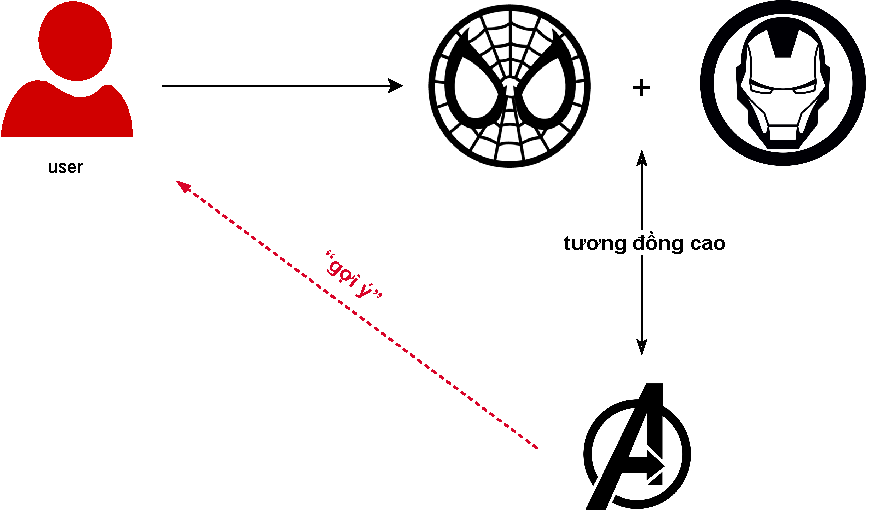
\includegraphics[width=0.6\textwidth]{CBF.pdf}
    \caption{Minh họa cách hoạt động của ``Content-Based Filtering'':
    mô hình gợi ý bộ phim có độ tương đồng cao với các bộ phim
    người dùng đã xem trước đó}
    \label{fig_CBF}
\end{figure}
Với hướng tiếp cận này, mô hình chỉ cần các thuộc tính mô tả của sản phẩm mà 
không đòi hỏi dữ liệu tương tác từ người dùng khác
vì các gợi ý là dành riêng cho từng cá nhân, do đó nó có khả năng nắm bắt tốt các sở thích
đặc biệt của người dùng.
Vì dựa trên ``tính tương đồng'' của sản phẩm, hệ thống có thể gợi ý một sản phẩm phù hợp với người dùng nhưng sản phẩm này có thể không được nhiều người dùng khác quan tâm.
Để áp dụng ``Content-Based Filtering'' cho từng loại dữ liệu cụ thể,
ta cần ``domain knowledge'' cho lĩnh vực đó để thiết kế mô hình.
Trong trường hợp các lĩnh vực có ít thông tin chi tiết về sản phẩm, hay các dữ liệu về sản phẩm thường không đầy đủ, rõ ràng thì 
hướng tiếp cận này sẽ tỏ ra không hiệu quả. 

Một hướng tiếp cận khác là tìm ra ``độ tương đồng'' giữa các người dùng với nhau, hay tìm ra được một nhóm người dùng
có cùng sở thích dựa trên dữ liệu tương tác của tất cả người dùng. Khi đó, để có thể gợi ý cho một người dùng cụ thể,
hệ thống sẽ tìm ra các sản phẩm không có trong lịch sử tương tác của người dùng đó, và đã được những người dùng ``tương đồng'' với họ tương tác trước đó,
thì hướng tiếp cận này được gọi là ``Collaborative Filtering'' (lọc cộng tác) (hình~\ref{fig_CF} mô tả hướng tiếp cận này).
\begin{figure}
    \centering
    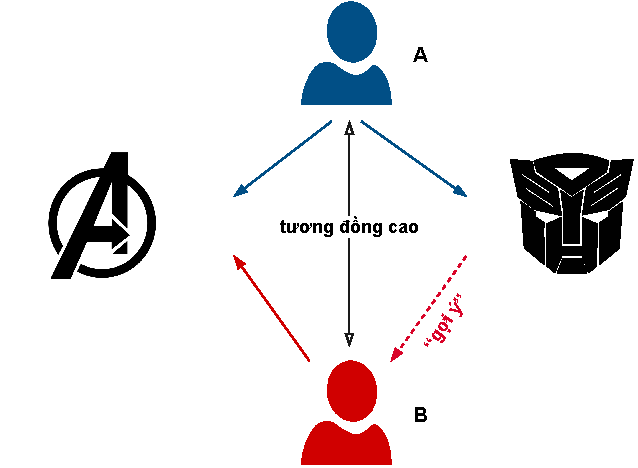
\includegraphics[width=0.6\textwidth]{CF.pdf}
    \caption{Minh họa cách hoạt động của ``Collaborative Filtering'': hai người dùng cùng xem một (hoặc nhiều) bộ phim 
    sẽ được hệ thống đánh giá là hai người dùng ``tương đồng'' nhau, khi đó một bộ phim được
    người dùng A xem sẽ được gợi ý cho người dùng B}
    \label{fig_CF}
\end{figure}
Đối với hướng tiếp cận ``Collaborative Filtering'', mô hình dựa vào lịch sử tương tác từ người dùng khác
và không dùng các thuộc tính mô tả của sản phẩm, do đó nó có khả năng tạo ra sự tình cờ cho người dùng:
hệ thống có thể gợi ý một sản phẩm ``tốt'' cho người dùng trong trường hợp sản phẩm đó có ít điểm tương đồng
so với các sản phẩm người dùng đã ``thích'' trước đó. Dữ liệu đầu vào của hướng tiếp cận này là các tương tác
của người dùng với các sản phẩm, do đó có thể áp dụng cho nhiều lĩnh vực khác nhau mà không cần thiết phải thay đổi cấu trúc hệ thống 
hoặc nếu có thì cũng không cần phải thay đổi quá nhiều.
Tuy nhiên, ``Collaborative Filtering'' gặp phải một vấn đề được gọi là ``khởi động nguội'' (``cold-start''),
đó là khi mà một người dùng mới đến với hệ thống thì hệ thống sẽ thường khó đưa ra được gợi ý tốt cho họ,
hoặc khi một sản phẩm được ít được người dùng tương tác, hệ thống thường sẽ không gợi ý sản phẩm đó cho những người dùng khác.

Ngoài ra, một hướng tiếp cận khác là ``Hybrid'', là sự kết hợp giữa hai hướng tiếp cận bên trên.
Trong giới hạn của khóa luận này, chúng tôi chỉ tập trung tìm hiểu về hướng tiếp cận ``Collaborative Filtering'' 
vì ba lý do chính là:
\begin{itemize}
\item ``Collaborative Filtering'' tổng quan hơn so với ``Content-Based Filtering''
- hướng tiếp cận cần ``domain knowledge'' để thiết kế hệ thống cho từng lĩnh vực cụ thể.
\item Với số lượng lớn và cùng với sự đa dạng của các ``sản phẩm'' hiện nay, tận dụng điều này, 
việc hệ thống gợi ý các sản phẩm đa dạng hơn dựa trên sở thích của các người dùng sẽ phù hợp hơn so với việc
đưa ra các sản phẩm tương đồng với nhau.
\item Ngoài ra, khi số lượng người dùng trên mạng Internet càng ngày càng tăng nhanh, thì ``collaborative filtering'' 
sẽ có được nhiều lợi thế hơn khi có thể kết hợp dữ liệu tương tác của các người dùng để đưa ra gợi ý.
\end{itemize}

Việc kết hợp các thông tin chi tiết về người dùng hay từ sản phẩm sẽ là một thông tin hữu ích cho việc xây dựng
một hệ thống gợi ý sản phẩm hiệu quả hơn. Nhưng đây là một điều không đơn giản bởi nó phụ thuộc vào ``domain knowledge'' ở từng lĩnh vực và chúng tôi để lại như một định hướng trong việc nghiên cứu và phát triển trong tương tai.

Phương pháp đầu tiên trong việc xây dựng một hệ thống gợi ý sản phẩm theo hướng tiếp cận ``Collaborative Filtering'' là thuật toán ``Matrix Factorization'' được giới thiệu bởi Hu \cite{MF}. Với ý tưởng là xây dựng một mô hình có khả năng ``tái tạo'' lại tương tác của người dùng, trong đó các tương tác được tái tạo cũng bao gồm các gợi ý cho họ.
Cho đến hiện nay, ``Matrix Factorization'' vẫn  là một phương pháp đơn giản nhưng vẫn mang lại kết quả cao.
Tuy nhiên, thuật toán này có các nhược điểm chí mạng mà khó có thể được áp dụng để xây dựng một hệ thống gợi ý sản phẩm quy mô lớn đó là số lượng tham số của mô hình tỉ lệ tuyến tính vào cả số lượng người dùng và số lượng sản phẩm.
Khi mà ngày nay, số lượng người dùng và sản phẩm tăng rất nhanh theo thời gian, ngoài ra sau khi huấn luyện mô hình, mô hình cần thực hiện các bước tối ưu đặc biệt để có thể gợi ý cho người dùng mới. 
Ngoài ra, ``Matrix Factorization'' vẫn còn hạn chế đó là mô hình này là một mô hình tuyến tính, do đó nó chưa có khả năng ``học'' được các ``đặc trưng phi tuyến'' của dữ liệu.
``Asymetric matrix factorization'' là một phương pháp cải tiến từ ``Matrix Factorization'' với ý tưởng rút trích các đặc trưng của người dùng thông qua các sản phẩm mà họ đã tương tác. Phương pháp này đã khắc phục được nhược điểm của ``Matrix Factorization'' khi mà số lượng tham số của mô hình giờ chỉ phụ thuộc vào số lượng sản phẩm có trong hệ thống. Trong thực tế, số lượng sản phẩm sẽ tăng chậm hơn đáng kể so với số lượng người dùng trong hệ thống thì khắc phục này sẽ là một điểm mạnh của ``Asymetric matrix factorization''. Ngoài ra nó cũng đã giảm bớt được chi phí để đưa ra dự đoán cho người dùng mới. Tuy nhiên, với hạn chế của các hàm tuyến tính nên phương pháp này vẫn chưa thực sự mạnh.
Ở công trình nghiên cứu \cite{AMF} của tác giả Steck đã chỉ ra rằng ``Asymetric Matrix Factorization'' có thể được xem như là một mô hình ``Auto-Encoder'' tuyến tính. ``Auto-Encoder'' là một mô hình học đặc trưng ẩn không giám sát. Mô hình này thường được sử dụng trong những tác vụ như rút trích đặc trưng hay giảm chiều dữ liệu, ... Dựa trên ý tưởng rằng, giả định tương tác của người dùng sẽ được ``phát sinh'' từ một ``đặc trưng ẩn'', ta có thể xem rằng ``đặc trưng ẩn'' này là sở thích của họ, và ta sẽ xây dựng một mô hình phát sinh được đặc trưng ẩn của người dùng từ dữ liệu tương tác của người dùng với hệ thống các sản phẩm. Sau đó đặc trưng ẩn này được sử dụng để đưa ra các gợi ý cho người dùng. Trong thời gian gần đây đã có nhiều nghiên cứu áp dụng mô hình ``Auto-Encoder'' trong bài toán xây dựng hệ thống gợi ý sản phẩm \cite{autorec,cdae,mvae} để có thể tận dụng sức mạnh của các hàm phi tuyến, cụ thể là sử dụng mạng nơ-ron với các hàm kích hoạt phi tuyến (là kiến trúc cơ bản của các mô hình được dùng huấn luyện trong lĩnh vực học máy) để có được một mô hình ``mạnh'' hơn so với các phương pháp tuyến tính trước đó.
``AutoRec'' \cite{autorec} được Sedhain giới thiệu tại hội nghị WWW2015, là mô hình được coi là đầu tiên trong việc sử dụng kiến trúc mô hình ``Auto-Encoder'' để đưa ra gợi ý cho người dùng bằng cách huấn luyện mô hình để tái tạo lại dữ liệu tương tác của người dùng sau khi trích xuất đặc trưng ẩn từ dữ liệu tương tác của họ. ``Collaborative denoising auto-encoders for top-n recommender systems'' \cite{cdae} (CDAE) được Wu cùng các cộng sự đề xuất nhằm hướng đến bài toán đưa ra gợi ý theo hướng xếp hạng và đưa ra ``top-N sản phẩm'' phù hợp nhất với người dùng hay nói cách khác là dự đoán tập các sản phẩm mà người dùng ``thích'' nhất. Mô hình này dã được xây dựng dựa trên ``AutoRec'' nhưng có các chỉnh sửa để phù hợp hơn với bài toán xây dựng hệ thống gợi ý sản phẩm khi mà ta quan tâm đến việc đưa ra xếp hạng các sản phẩm phù hợp với người dùng thay vì tái tạo lại tương tác của họ. 
Ngoài ra, việc thêm ``nhiễu'' vào dữ liệu huấn luyện của CDAE giúp mô hình ``Auto-Encoder'' phải học cách trích xuất các đặc trưng ẩn tốt và tạo ra gợi ý thay vì chỉ cố gắng tái tạo lại dữ liệu tương tác ``giống'' đầu vào nhất có thể, cũng như ``nhiễu'' sẽ giúp quá trình huấn luyện mạng nơ-ron với hàm kích hoạt phi tuyến tránh được tình trạng ``over-fitting'' (tình trạng học ``tủ'' trên tập dữ liệu huấn luyện, dẫn đến mô hình đạt được kết quả thấp trên các tập dữ liệu kiểm định).

% Ngoài ra, CDAE còn cải tiến từ ``AutoRec'' đó là thêm ``nhiễu'' vào dữ liệu huấn luyện nhằm giúp mô hình tránh được tình trạng ``Over-fitting'' (là trình trạng mà mô hình học ``tủ'' trên tập dữ liệu được huấn luyện nên mô hình đạt kết quả thấp trên các tập dữ liệu kiểm định), thường gặp phải khi huấn luyện mạng nơ-ron với hàm kích hoạt phi tuyến.

Một trong những phương pháp nổi bật nhất tới thời điểm hiện tại trong việc sử dụng kiến trúc mô hình ``Auto-Encoder'' để xây dựng mô hệ thống gợi ý sản phẩm là ``Variational Autoencoder for Collaborative Filtering''\cite{mvae} được giới thiệu bởi tác giả Liang cùng các cộng sự công bố tại hội nghị ``International World Wide Web Conference Committee 2018''. 
Đây là một phương pháp sử dụng mô hình ``Variational Auto-encoder'' (VAEs) - một biến thể của mô hình ``Auto-Encoder'' cơ bản để có thể xây dựng một hệ thống gợi ý sản phẩm hiệu quả. ``Variational Auto-encoder'' đã đạt được một số thành công nhất định trong bài toán xây dựng hệ thống gợi ý. Theo nghiên cứu của Dacrema \cite{dacrema2019we}, mô hình được đề xuất trong \cite{mvae} đạt được các kết quả tốt trong việc gợi ý và xếp hạng. Trong khóa luận này, chúng tôi tìm hiểu và cài đặt lại mô hình được đề xuất trong bài báo \cite{mvae}, và thực hiện một số thí nghiệm nhằm phân tích khả năng học của mô hình.

%----------------------Add in---------------------%
Với một mô hình ``Auto-encoder'' nói chung, ta thường chỉ quan tâm đến việc thu được véc-tơ biểu diễn ẩn có thể hiện đúng tính chất của dữ liệu đầu vào sau quá trình huấn luyện. Ứng dụng của mô hình này thường là trích xuất các đặc trưng ẩn hoặc giảm chiều dữ liệu - đồng nghĩa với việc tái tạo dữ liệu là một quá trình phụ trợ cho việc huấn luyện mô hình. Nghĩa là mô hình sẽ tái tạo hoặc trích xuất được các ``đặc trưng ẩn'' của dữ liệu mà không thể sinh ra dữ liệu mới. 
Ứng dụng của ``Auto-encoder'' trong các bài báo \cite{autorec,cdae} trong hệ thống gợi ý là cố gắng tái tạo lại ``đặc trưng ẩn của người dùng'', từ đó cũng sinh ra các gợi ý.
Vô tình, ý tưởng này dẫn đến rằng việc đưa ra gợi ý không phải là mục đích chính của mô hình, mà gợi ý được tạo một cách gián tiếp thông qua việc tái tạo lại dữ liệu.
Với bài toán xây dựng hệ thống gợi ý, việc tạo ra các gợi ý cho người dùng phải là một việc được ưu tiên. Mô hình VAEs với ``đặc trưng ẩn'' được phát sinh từ một phân phối xác suất, và được xem như một mô hình có thể phát sinh dữ liệu mới từ ``đặc trưng ẩn''. Khi ứng dụng trong bài toán xây dựng hệ thống gợi ý, việc phát sinh dữ liệu mới này tương đồng với việc tạo ra các gợi ý, đồng thời cũng vẫn giữ được tính chất của ``Auto-encoder'' trong bài toán này là tương tác người dùng được phát sinh từ một ``đặc trưng ẩn'' (cũng chính là sở thích của người dùng).


Hơn nữa, với nền tảng của mô hình VAEs dựa trên phương pháp ``Variational Inference'' trong lĩnh vực xác suất thống kê. ``Variational Inference'' dùng để suy diễn dữ liệu ẩn từ dữ liệu ta quan sát được, hay cụ thể trong bài toán này là suy diễn ác ``đặc trưng ẩn'' dựa vào dữ liệu quan sát được là các tương tác của người dùng. 
Đặc điểm của phương pháp này là có thể áp dụng tốt cho dữ liệu thưa, có nghĩa là đối với ``dữ liệu quan sát được'' bị hạn chế thì việc ``suy diễn'' dữ liệu vẫn đạt được kết quả tốt. 
Trong hệ thống gợi ý, tính chất của dữ liệu thường là thưa, do mỗi người dùng chỉ tương tác với một lượng nhỏ sản phẩm trên toàn hệ thống, từ đó việc suy diễn trở nên hiệu quả trong hệ thống gợi ý.

Cùng với mục tiêu đánh giá xếp hạng các sản phẩm, với mục đích sản phẩm liên quan đến người dùng hơn được ưu tiên gợi ý hơn. Tác giả Liang đã giới thiệu ``Multinomial log-likelihood'' cho việc tính toán độ lỗi. Với tính chất trả về một giá trị xác suất cho mỗi sản phẩm, và tổng giá trị xác suất trên toàn bộ sản phẩm là 1. Ngoài ra ``likelihood'' sẽ khuyến khích mô hình đánh giá các sản phẩm là một giá trị lớn hơn 0. Các sản phẩm sẽ phải ``cạnh tranh'' với nhau để có được xác suất cao hơn. Tuy không được sử dụng nhiều trong lĩnh vực xây dựng hệ thống gợi ý sản phẩm, thay vào đó, ``Multinomial log-likelihood'' lại thường được sử dụng nhiều trong các lĩnh vực về mô hình ngôn ngữ (Language models) hay về các bài toán trong lĩnh vực kinh tế (Ecomomics) nhưng chúng tôi tin rằng ``Multinomial log-likelihood'' sẽ là một lựa chọn phù hợp trong lĩnh vực xây dựng hệ thống gợi ý sản phẩm.

Mặc dù mô hình được tác giả Liang đề xuất ở bài báo \cite{mvae} không phải là mô hình đạt được kết quả tốt nhất hiện nay trong việc xây dựng hệ thống gợi ý sản phẩm, tuy nhiên với những lí do nêu trên, chúng tôi tin rằng kiến thức nền tảng để xây dựng mô hình này bao phủ về lĩnh vực học máy cũng như là kiến thức về mô hình xác suất. Vậy nên chúng tôi quyết định sẽ tập trung tìm hiểu mô hình này. 


%--------------------------------------------------%

% Lý do đầu tiên mà chúng tôi quyết định tìm hiểu về mô hình này cũng như là điểm khác biệt của VAEs so với các phương pháp đã được kể đến ở trên đó là đặc trưng ẩn được phát sinh là một phân phối xác suất thay vì là ``một điểm dữ liệu cố định'' (``Auto-Encoder'' và ``Denosing Auto-Encoder'' sẽ nhận dữ liệu đầu vào ở chiều không gian ``cao'' và trích xuất đặc trưng ẩn là một điểm dữ liệu ở chiều không gian ``thấp'' hơn mà vẫn thể thể hiện được ``tính chất'' của dữ liệu ban đầu).
% Việc đặc trưng ẩn là một phân phối xuất sẽ giúp cho mô hình có thể sử dụng dặc trưng ẩn này để phát sinh dữ liệu, ứng dụng với bài toán ta đang quan tâm đó chính là sử dụng sở thích nắm bắt được từ các người dùng để đưa ra gợi ý cho họ.
% Nền tảng của VAEs đó là dựa trên phương pháp ``Variational Inference'', một phương pháp trong lĩnh vực xác suất thống kê. 
% Phương pháp này thường được dùng để suy diễn ``dữ liệu ẩn'' dựa trên những ``dữ liệu ta quan sát được''. Đặc điểm của phương pháp này là có thể áp dụng tốt cho dữ liệu thưa, có nghĩa là đối với ``dữ liệu quan sát'' được bị hạn chế thì việc ``suy diễn'' dữ liệu vẫn đạt được kết quả tốt. 
% Ở đây, trong bài toán xây dựng hệ thống gợi ý sản phẩm, dữ liệu tương tác của người dùng sẽ được xem là dữ liệu quan sát được và đặc trưng ẩn là ``dữ liệu ẩn'' mà ta không quan sát được. 
% Đặc biệt ở đây, đối với bài toán xây dựng hệ thống gợi ý sản phẩm thì thông thường mỗi người dùng chỉ tương tác với một lượng tỉ lệ nhỏ các sản phẩm so với toàn bộ sản phẩm có trong hệ thống, do đó việc áp dụng phương pháp ``Variational Inference'' hay nói cách khác là VAEs sẽ phù hợp với bài toán xây dựng hệ thống gợi ý sản phẩm dựa trên ý tưởng phát sinh tương tác của người dựa vào đặc trưng ẩn của người dùng.
% Bên cạnh đó, để có thể xây dựng một mô hình giải quyết giải quyết vấn đề mà hệ thống gợi ý sản phẩm quan tâm đó là có thể đưa ra được tập các sản phẩm có khả năng cao sẽ phù hợp với người dùng, mục đích này khác hoàn toàn với việc tái tạo lại dữ liệu hay nói cách khác là tái tạo lại tương tác của người dùng.
% Với mục tiêu để mô hình thể hiện được rõ khả năng mà một sản phẩm có phù hợp với người dùng hay không thì tác giả Liang đã sử dụng hàm ``Multinomial log-likelihood'' (một phương pháp đánh giá bộ tham số của mô hình với giả định dữ liệu tương tác của người dùng tuân theo một phân phối đa thức). 
% ``Multinomial log-likelihood'' sẽ khiến kết quả trả về từ mô hình thể hiện ``giá trị độ lớn về xác suất''. Với ``multinomial log-likelihood'' các sản phẩm sẽ phải ``cạnh tranh'' với nhau để có thể đạt được xác suất được chọn cao hơn (vì kết quả trả về sẽ phải ràng buộc là tổng kết quả  ``xác suất'' trả về sẽ bằng 1 hay xác suất được chọn của các sản phẩm trả về từ mô hình sẽ có tổng bằng 1).
% Tuy không được sử dụng nhiều trong lĩnh vực xây dựng hệ thống gợi ý sản phẩm, thay vào đó, ``Multinomial log-likelihood'' lại thường được sử dụng nhiều trong các lĩnh vực về mô hình ngôn ngữ (Language models) hay về các bài toán trong lĩnh vực kinh tế (Ecomomics) nhưng chúng tôi tin rằng ``Multinomial log-likelihood'' sẽ là một lựa chọn phù hợp trong lĩnh vực xây dựng hệ thống gợi ý sản phẩm.

% Cuối cùng, một điểm đặc biệt của phương pháp này đó là tác giả đã đề xuất thêm một siêu tham số để kiểm soát việc đánh đổi giữa việc tối thiểu độ lỗi trong việc mô hình hóa dữ liệu và việc đảm bảo đặc trưng ẩn được phát sinh tuân theo phân phối xác suất được giả định từ mô hình. 
% Siêu tham số là một tham số được chỉ định bởi lập trình viên cho mô hình thay vì mô hình học phải học như các tham số thông thường.
% Nguyên nhân dẫn đến việc cần phải có một siêu tham số để kiểm soát được việc đánh đổi nói trên là vì với việc xây dựng một hệ thống gợi ý sản phẩm thì chúng ta sẽ quan tâm tới việc mô hình hoá dữ liệu nhiều hơn là việc đảm bảo đặc trưng ẩn sẽ tuân theo phân phối xác suất. 
% Nói một cách khác, thì việc mô hình hoá dữ liệu sẽ đảm bảo rằng đặc trưng ẩn có được từ mô hình sẽ thể hiện được cho dữ liệu ban đầu, hay trong bài toán xây dựng hệ thống gợi ý thì điều này đảm bảo mô hình sẽ nắm bắt được xu hướng sở thích giữa các người dùng nhưng nếu mô hình chỉ tập trung để mô hình hoá dữ liệu thì mô hình sẽ bị giới hạn lại thành việc tái tạo lại tương tác của người dùng.
% Còn về việc đảm bảo tính chất về phân phối xác suất sẽ giúp cho đặc trưng có thể phát sinh được dữ liệu một cách hợp lý, nếu quá tập trung để đảm bảo điều này thì mô hình sẽ khó nắm  bắt được sở thích chung giữa các người dùng, ngược lại, nếu bỏ qua tính chất này, thì đặc trưng ẩn sẽ khó có thể đưa ra được những sản phẩm không nằm trong lịch sử tương tác mà phù hợp với người dùng.
% Do vậy, khi xây dựng hệ thống gợi ý sản phảm thì ta sẽ cần phải kiểm soát được việc đánh đổi này thì hệ thống gợi ý mới có thể hoạt động hiệu quả hơn.

% Mặc dù không phải là mô hình đạt được kết quả tốt nhất hiện nay trong việc xây dựng hệ thống gợi ý sản phẩm, tuy 
% nhiên kiến thức nền tảng để xây dựng mô hình này bao phủ về lĩnh vực học máy cũng như là kiến thức về mô hình xác suất.
% Với những lợi điểm như trên, thì chúng tôi đã quyết định sẽ tập trung tìm hiểu mô hình được tác giả Liang đề xuất ở bài báo \cite{mvae}. 


% Tuy có những lợi điểm trên nhưng trong thực tế thì để VAEs có thể ``hoạt động'' tốt với bài toán xây dựng hệ thống gợi ý sản phẩm thì không dễ.
% Để VAEs ``hoạt động'', có hai việc cần phải giải quyết là: (i) kết quả trả về từ mô hình sẽ là tập các sản phẩm được dự đoán là có khả năng thể hiện sự phù hợp với người dùng chứ việc tái tạo lại dữ liệu ban đầu không phải mục tiêu chính trong việc xây dựng hệ thống gợi ý sản phẩm và (ii) đánh đổi giữa việc tái tạo lại dữ liệu và việc đặc trưng ẩn được phát sinh tuân theo giả định về phân phối xác suất của mô hình.
% Để kết quả trả về từ mô hình là tập các sản phẩm có ``xác suất'' hay thể hiện sự phù hợp với người dùng thì chúng tôi sử dụng hàm 
% % ``Multinomial log-likelihood'' (hàm log-likelihood là hàm số dùng để đánh giá bộ trọng số của mô hình), 
% ``Multinomial log-likelihood'' (một phương pháp đánh giá bộ tham số của mô hình với giả định dữ liệu tương tác của người dùng tuân theo một phân phối đa thức),
% ``Multinomial log-likelihood'' sẽ khiến kết quả trả về từ mô hình thể hiện ``giá trị độ lớn về xác suất''. Với ``multinomial log-likelihood'' các sản phẩm sẽ phải ``cạnh tranh'' với nhau để có thể đạt được xác suất được chọn cao hơn (vì kết quả trả về sẽ phải ràng buộc là tổng kết quả  ``xác suất'' trả về sẽ bằng 1 hay xác suất được chọn của các sản phẩm trả về từ mô hình sẽ có tổng bằng 1).
% Tuy không được sử dụng nhiều trong lĩnh vực xây dựng hệ thống gợi ý sản phẩm, thay vào đó, ``multinomial log-likelihood'' lại thường được sử dụng nhiều trong các lĩnh vực về mô hình ngôn ngữ (Language models) hay về các bài toán trong lĩnh vực kinh tế (Ecomomics) nhưng chúng tôi tin rằng ``multinomial log-likelihood'' sẽ là một lựa chọn phù hợp trong lĩnh vực xây dựng hệ thống gợi ý sản phẩm.
% Về vấn đề đánh đổi giữa việc tối thiểu độ lỗi trong việc mô hình hóa dữ liệu và việc đảm bảo đặc trưng ẩn được phát sinh tuân theo phân phối xác suất được giả định từ mô hình thì chúng tôi sử dụng một siêu tham số mới để kiểm soát việc đánh đổi này.
% Tuy nhiên, với việc sử dụng siêu tham số để kiểm soát về việc đánh đổi nói trên thì ta sẽ cần phải giải quyết thêm một vấn đề khác đó là việc lựa chọn siêu tham số phù hợp cho mô hình. Siêu tham số là một tham số được chỉ định bởi lập trình viên cho mô hình thay vì mô hình học phải học như các tham số thông thường.
% Thường thì việc lựa chọn siêu tham số cho các mô hình học là một công đoạn tốn thời gian và phiền phức khi mà ta cần phải chạy mô hình nhiều lần với các bộ siêu tham số khác nhau để chọn ra được siêu tham số để mô hình có kết quả tốt.
% Như vậy, có hai câu hỏi được trả lời để mở rộng VAEs cho bài toán xây dựng hệ thống gợi ý sản phẩm là: (i) tại sao Multinomial log-likelihood lại phù hợp hơn với bài toán xây dựng hệ thống gợi ý sản phẩm?; (ii) làm sao để tối ưu được việc đánh đổi giữa độ lỗi trong việc mô hình hoá dữ liệu và việc đảm bảo đặc trưng ẩn có được từ mô hình tuân theo một phân phối xác suất được giả định. Cụ thể:
% \begin{itemize}
%     \item Chúng tôi tiến thành thực hiện huấn luyện mô hình VAE với hàm ``multinomial log-likelihood'' và chúng tôi gọi VAEs với hàm ``multinomial log-likelihood'' là Mult-VAEs. Bên cạnh đó, chúng tôi cũng thực hiện huấn luyện VAEs để so sánh hàm log-likelihood này với các hàm log-likelihood thường được áp dụng khi huấn luyện VAEs là Gaussian log-likelihood và Logistic likelihood.
%     \item Hơn nữa, chúng tôi cũng đề xuất một siêu tham số để kiểm soát việc đánh đổi thường gặp khi huấn luyện VAEs. Và phương pháp để lựa chọn cho siêu tham số này thay vì phải thực hiện huấn luyện với các gía trị siêu tham số khác nhau.
% \end{itemize}

% Với hai thành phần trên (sử dụng hàm multinomal log-likelighood và siêu tham sô kiểm soát sự đánh đổi trong lúc huấn luyện), kết quả thí nghiệm trên các bộ dữ liệu lớn trong tác vụ xây dựng hệ thống gợi ý sản phẩm như Movielens-20M và Million Song Datasets cho thấy Mult-VAEs đạt được kết quả ấn tượng, ngoài ra việc sử dụng hàm multinomial log-likelihood cho kết quả tốt hơn so với các hàm log-likelihood thông dụng khác.


Phần còn lại của khóa luận được trình bày như sau:

\begin{itemize}
    \item Chương~\ref{Chapter2} trình bày sơ lược về mô hình ``Auto-Encoder'' và các kiến thức nền tảng của mô hình ``Variational Auto-Encoder''.
    \item Chương~\ref{Chapter3} trình bày về cách áp dụng mô hình ``Variational Auto-Encoder'' cùng với hàm lỗi ``Multinomial log-likelihood'' cho bài toán xây dựng hệ thống gợi ý. Bên cạnh đó, chương này cũng phân tích các hạn chế của mô hình đồng thời đề xuất phương pháp giúp giải quyết các hạn chế đó. Chương này là phần chính của khóa luận.
    \item Chương~\ref{Chapter4} trình bày về các thí nghiệm và các kết quả đạt được.
    \item Cuối cùng, tổng kết và hướng phát triển được trình bày ở chương~\ref{Chapter5}.
\end{itemize}



\chapter{Kiến thức nền tảng}
\label{Chapter2}
\graphicspath{{Chapter2/Chapter2Figs}}
\justifying

\setlength{\parindent}{6.5ex}
\textit{Trong chương này, đầu tiên chúng tôi sẽ trình bày về mô hình 
``Auto-Encoder'' (AE), một mạng nơ-ron được dùng để học đặc trưng ẩn dựa trên
phương pháp học không giám sát.
Kế tiếp, chúng tôi giới thiệu và trình bày về mô hình ``Variational Auto-Encoder'' (VAE) và các nền tảng xác suất của nó. Các nền tảng xác suất bao gồm: Variational Inference - một phương pháp suy diễn dữ liệu hiệu quả - và Maximum Likelihood Estimation - một phương pháp để ước lượng một bộ tham số tốt cho mô hình.
}


% \textit{Bên cạnh đó, chúng tôi sẽ trình bày về ``Log-likelihood fuctions'' - 
% là phép đo mức độ học của mô hình dựa trên các dữ liệu ta quan sát được 
% cũng như các lựa chọn Log-likelihood fucntion cho các bài toán học máy hiện nay.}
% 7->10; 15->20; 15->20; 10->15; 2 (~60)

\section{Mô hình rút trích đặc trưng ẩn ``Auto-Encoder''}
\label{chap2/sec1}
Mô hình ``Auto-Encoder'' (AE) là một mạng nơ-ron truyền thẳng được huấn luyện
để cố gắng sao chép đầu vào của nó thành đầu ra với mục đích trích xuất được các đặc trưng ẩn. Bên trong ``Auto-Encoder''
có một lớp ẩn \textbf{\textit{h}} mô tả đặc trưng ẩn, gọi là véc-tơ biểu diễn ẩn đại diện cho đầu vào của nó.

Kiến trúc của một ``Auto-Encoder'' (được minh họa trong hình~\ref{fig_AE}) bao gồm hai phần:
\begin{itemize}
    \item Bộ mã hóa (encoder) ánh xạ véc-tơ đầu vào sang véc-tơ biểu diễn ẩn: 
    \begin{center}
        \begin{math}
            \centering
            \textbf{\textit{h}} = f(x)
        \end{math} 
            
    \end{center}
    \item Bộ giải mã (decoder) có nhiệm vụ cố gắng tái tạo lại véc-tơ đầu vào từ véc-tơ biểu diễn ẩn:
    \begin{center}
        \begin{math}
            \hat{x} = g(\textbf{\textit{h}}) = g(f(x))
        \end{math}
    \end{center}
\end{itemize}

\begin{figure}
    \centering
	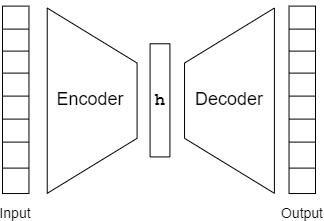
\includegraphics[width=0.6\textwidth]{AE.png}
    \caption{Minh họa ``Auto-Encoder''}
    \label{fig_AE}
\end{figure}

``Auto-Encoder'' được huấn luyện bằng cách cực tiểu hóa hàm lỗi là độ sai lệch giữa dữ liệu được tái tạo
với dữ liệu đầu vào. 
\begin{equation}
\label{AE_loss}
    L(x, g(f(x)))
\end{equation}
Các hàm để tính độ lỗi thường được dùng là ``Mean-square error'' hoặc ``Binary cross-entropy''.
Tương tự như các mạng nơ-ron khác, ``Auto-Encoder'' có thể được huấn luyện bằng phương pháp ``Gradient-descent''
với thuật toán lan truyền ngược (``back-propagation'').



Khi thiết kế mô hình, kiến trúc của encoder, decoder
và kích thước của véc-tơ \textbf{\textit{h}} được xem như những siêu tham số của mô hình.
Bằng các cách thiết lập khác nhau, mô hình sẽ có những tính chất khác nhau. 
``Auto-Encoder'' với encoder và decoder là những hàm phi tuyến (cụ thể là mạng nơ-ron với hàm kích hoạt phi tuyến)
với khả năng tính toán quá mạnh hay trường hợp kích thước của véc-tơ \textbf{\textit{h}}
lớn hơn hoặc bằng so với véc-tơ đầu vào sẽ dẫn đến mô hình chỉ học cách sao chép thay vì trích xuất các đặc trưng ẩn từ dữ liệu. 

Thông thường, một ``Auto-Encoder'' sao chép một cách ``hoàn hảo'' đầu vào thành đầu ra
sẽ không có nhiều ý nghĩa. Thay vào đó, ``Auto-Encoder'' được thiết kế với các ràng buộc để không thể
học cách sao chép ``hoàn hảo'' mà chỉ có thể sao chép gần đúng, từ đó ta hy vọng quá trình 
huấn luyện ``Auto-Encoder'' sẽ thu được véc-tơ biểu diễn ẩn có những thông tin hữu ích.

Từ véc-tơ biểu diễn ẩn thu được trong quá trình huấn luyện ``Auto-Encoder'', ta có thể áp dụng mô hình này
như một mô hình trích xuất đặc trưng ẩn từ dữ liệu, làm đầu vào cho các tác vụ khác. 
Hoặc véc-tơ biểu diễn ẩn này có thể áp dụng được trong các tác vụ giảm chiều dữ liệu hỗ trợ cho các tác vụ
lưu trữ, truy vấn, tìm kiếm.

    \subsection{``Undercomplete Auto-Encoder''}
    \label{chap2/subsec11}
    Như đã trình bày trước đó, việc sao chép đầu vào thành đầu ra của ``Auto-Encoder'' không mang nhiều ý nghĩa.
    Với mục đích thu được véc-tơ biểu diễn ẩn của dữ liệu thông qua quá trình huấn luyện, ta cần các ràng buộc để có được \textbf{\textit{h}}
    nhận các thuộc tính hữu ích khi thiết kế mô hình.
    
    Một cách ràng buộc để mô hình có thể học được các đặc trưng ẩn từ dữ liệu
    là giới hạn véc-tơ đặc trưng ẩn \textbf{\textit{h}} có kích thước nhỏ hơn đáng kể so với véc-tơ đầu vào;
    tính chất này được gọi là ``under-complete''.
    
    Mô hình ``Auto-Encoder'' với kích thước \textbf{\textit{h}} nhỏ hơn đáng kể so với kích thước của véc-tơ đầu vào
    được gọi là ``Undercomplete Auto-Encoder''. Việc giới hạn này sẽ buộc mô hình phải nắm bắt các đặc trưng
    nổi bật nhất. Đây cũng là kiến trúc đa số các mô hình ``Auto-Encoder'' thường hay được sử dụng.

    Quá trình huấn luyện ``Undercomplete Auto-Encoder'' cũng giống với mô hình ``Auto-Encoder'',
    ta cần cực tiểu hóa hàm lỗi (công~thức~\ref{AE_loss}) là độ sai lệch giữa dữ liệu được tái tạo
    với dữ liệu đầu vào.

    ``Undercomplete Auto-Encoder'' là mô hình tốt để sử dụng cho các tác vụ tiêu biểu của ``Auto-Encoder'' truyền thống
    như trích xuất đặc trưng, giảm chiều dữ liệu 
    bởi vì tính chất ``under-complete'' của mô hình giúp dễ dàng thu được véc-tơ biểu diễn ẩn mang những thông tin hữu ích.


    \subsection{Biến thể của Auto-Encoder: ``Denoising Auto-Encoder''}
    \label{chap2/subsec12}
    
    Hàm lỗi của một ``Auto-Encoder'' thông thường sẽ ``phạt'' một mức nhất định với các mẫu dữ liệu được tái tạo lại
    khác với dữ liệu đầu vào. Điều này vô hình chung khuyến khích việc 
    $ f \circ g $ là một hàm đồng nhất nếu khả năng tính toán của $f$ và $g$ cho phép. Nói đơn giản hơn, điều này là việc mô hình sao chép ``hoàn hảo'' đầu vào thành đầu ra của nó.
    Khi đó, véc-tơ biểu diễn ẩn sẽ không có các thông tin hữu ích. 

    Bằng cách thay đổi cách tính toán độ lỗi khi tái tạo lại, cụ thể là thêm nhiễu vào véc-tơ đầu vào, 
    sau đó tính toán độ lỗi là đầu ra được mô hình tái tạo lại so với đầu vào ban đầu như sau:
    \begin{equation}
        L(x, g(f(\tilde{x})))
    \end{equation}
    với 
    \begin{math} \tilde{x} \end{math}
    là véc-tơ đầu vào 
    \begin{math}
        x
    \end{math} 
    được thêm một độ nhiễu, ta có được mô hình ``Denoising Auto-Encoder'' (DAE) (hình~\ref{fig_DAE}). 
    \begin{figure}
        \centering
        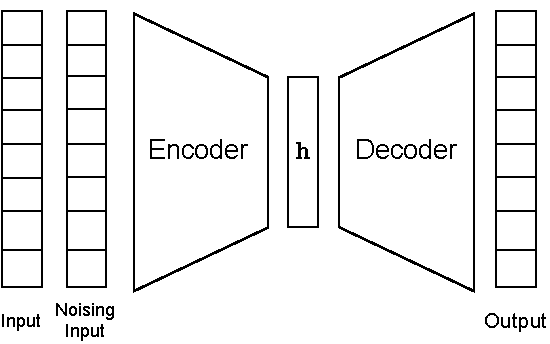
\includegraphics[width=0.6\textwidth]{DAE.pdf}
        \caption{Minh họa ``Denoising Auto-Encoder''}
        \label{fig_DAE}
    \end{figure}
    
    ``Denoising Auto-Encoder'' phải học cách khử độ nhiễu đã được thêm vào véc-tơ đầu vào, giảm khả năng sao chép của mô hình.

\section{Mô hình phát sinh dữ liệu ``Variational Auto-Encoder''} \label{chap2/sec2}
        \begin{figure}
            \centering
            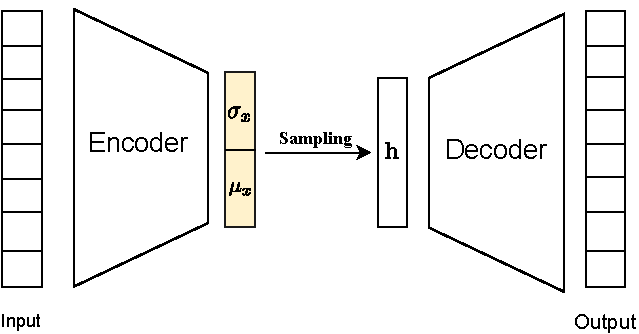
\includegraphics[width=0.6\textwidth]{VAE.pdf}
            \caption{Minh họa ``Variational Auto-Encoder''}
            \label{fig_VAE}
        \end{figure}
        ``Variational Auto-Encoder'' (VAE) là một biến thể đặc biệt của ``Auto-Encoder'' cơ bản (được minh họa trong hình~\ref{fig_VAE}). 
        VAE ngoài là một mô hình rút trích đặc trưng ẩn dựa trên phương pháp học không giám sát, còn là một mô hình phát sinh dữ liệu hiệu quả. 
        Phát sinh dữ liệu là việc mô hình có khả năng tạo ra những điểm dữ liệu `mới' dựa trên đặc trưng ẩn đã học được.
        Đây là một điểm khác biệt so với mô hình ``Auto-Encoder'' khi mà đặc trưng ẩn học từ ``Auto-Encoder'' cơ bản không thể được sử dụng để phát sinh. 
        Điều tạo nên sự khác biệt này là bởi đặc trưng ẩn có được từ VAE là một phân bố chứ không phải là một điểm dữ liệu cụ thể. 
        ``Auto-Encoder'' hay kể cả ``Denosing Auto-Encoder'', việc nhận dữ liệu đầu vào và trích xuất đặc trưng ẩn đều có thể được xem như là một phép chiếu dữ liệu ở chiều không gian cao lên một chiều không gian thấp hơn (thông thường thì kích thước của véc-tơ biểu diễn ẩn của một ``Auto-Encoder'' sẽ có tính chất ``under-complete'' như đã đề cập ở phần~\ref{chap2/subsec11}). 
        Do đó, ta có thể xem đặc trưng ẩn này như là một điểm dữ liệu ở một chiều không gian khác với số chiều thấp hơn thể hiện cho dữ liệu ban đầu. 
        Mặt khác, với VAE thì đặc trưng ẩn không còn là một điểm dữ liệu, thay vào đó sẽ là một ``phân phối xác suất''. 
        Phân phối xác suất thể hiện cho phân bố của một đại lượng, một biến ngẫu nhiên nào đó.
    
        Tuy nhiên, để làm rõ được sự hiệu quả của VAE trong việc phát sinh đặc trưng và phát sinh dữ liệu từ đặc trưng thì ta cần phải xét qua góc nhìn xác suất của mô hình này.
        Bản chất của một mô hình VAE là một mô hình đồ thị (graphical models) - là một mô hình dùng để giải thích các mối quan hệ giữa các biến ngẫu nhiên trong xác suất thống kê. Và nền tảng của mô hình là ``Variation Inference'' - là một phương pháp cũng thuộc lĩnh vực xác suất thống kê với mục đích có thể ``giải thích'' được dữ liệu mà ta không quan sát được từ những dữ liệu mà ta đã có. Tận dụng sức mạnh của mạng nơ-ron trong lĩnh vực học máy, các hàm số xác suất được thay thành các mạng nơ-ron. Và thông qua việc huấn luyện mô hình để tìm ra bộ trọng số tốt nhất để giải quyết bài toán được giả định mà mô hình cần giải quyết. 

        Do sự liên hệ chặt chẽ với lĩnh vực xác suất, ở mục này, chúng tôi sẽ trình bày về nền tảng xác suất liên quan với mô hình ``Variational Auto-Encoder'', bao gồm các khái niệm, định lý trong lĩnh vực xác suất thống kê để có thể dễ dàng trình bày nội dung của VAE ở mục tiếp theo, cũng như là cách huấn luyện cho mô hình VAE. 
        

    \subsection{Nền tảng xác suất của mô hình} \label{chap2/subsec21}
        
        Với sự tăng nhanh về số lượng dữ liệu có trên các nền tảng số thì nhu cầu cần một phương pháp có thể phân tích dữ liệu một cách tự động đang  càng ngày càng tăng theo.
        Mục tiêu của học máy đó là phát triển các phương pháp mà có thể tự động phát hiện các mẫu ``pattern'' trong dữ liệu.
        Các mô hình học máy tìm được những ``pattern'' này thông qua việc tìm các bộ tham số phù hợp với mô hình.
        Sau đó sử dụng những ``pattern'' vừa khám phá được để có thể dự đoán dữ liệu trong tương lai hoặc để thực hiện các mục đích khác như đưa ra các quyết định.
        Lý thuyết xác suất (``probability theory'') có thể được áp dụng cho bất kỳ vấn đề nào liên quan đến ``những điều chưa chắc chắn''. 
        Trong máy học, ``những điều chưa chắc chắn'' có thể là những sự thay đổi trong dữ liệu mà chúng ta chưa biết trước được, hay là những bộ tham số của mô hình.
        Gọi là chưa chắc chắn bởi vì ta không biết trước được và cũng không quan sát được về những điều này và ta không thể khẳng định hoàn toàn về những điều đó.
        Mô hình sẽ hoạt động như thế nào khi dữ liệu thay đổi? Liệu bộ tham số hiện tại của mô hình đã đủ tốt?
        Do đó học máy có liên quan khá là gần gũi với lĩnh vực xác suất thống kê và khai thác dữ liệu.

        
        Trên lý thuyết thì có ít nhất hai cách diễn giải của xác suất: ``diễn giải tần suất'' (frequentist interetation) và ``diễn giải bayesian''. Ở cách diễn giải thứ nhất thì xác suất được thể hiện thông qua việc thực hiện các thí nghiệm nhiều lần. Ví dụ như nếu ta thực hiện thí nghiệm tung đồng xu thì ta kì vọng rằng việc đồng xu xuất hiện mặt ngửa khoảng một nửa lần trong quá trình thực hiện. Còn ở cách diễn giải bayesian của xác suất thì thường được sử dụng để định lượng về ``những điều chưa chắc chắn''. Vậy nên ở góc nhìn này sẽ liên quan đến các thông tin hơn là việc lặp lại các thí nghiệm. Một trong những ưu điểm của cách diễn giải này đó là nó có thể được sử dụng để mô hình ``những điều chưa chắc chắn'' của sự việc/sự kiện mà ta đang quan tâm đến mà không có tần suất xuất dài hạn. Ví dụ liên hệ với các bài toán trong lĩnh vực học máy như chúng ta nhận một email và ta quan tâm đến việc tính phân phôi xác suất mà email vừa nhận là spam; hay trong bài toán chúng ta nhận thấy được một vật thể thông qua màn hình radar và ta muốn tính phân phối xác suất theo vật thể vừa được phát hiện chính xác là gì? một con chim, hay máy bay? Trong những trường hợp trên thì ý tưởng việc lặp lại các thí nghiệm sẽ không giúp ích cho chúng ta trong việc giải quyết các vấn đề nhưng với Bayesian thì điều này khá là tự nhiên và có thể được áp dụng để giải quyết bất kỳ vấn đề nào liên quan tới những ``điều không chắc chắn''.
        
        \subsubsection{Định lý Bayes và ứng dụng trong lĩnh vực học máy}
        Trong lĩnh vực ``máy học'' và ``thống kê Bayesian'', chúng ta thường quan tâm đến việc thực hiện các phép suy diễn dữ liệu ẩn ta không quan sát được khi cho trước các dữ liệu ta quan đã quan sát được.
        Ví dụ như ứng dụng một mô hình học máy trong việc phát hiện sản phẩm lỗi, khi ta đã có ghi nhận lại một số lượng dữ liệu mô tả của sản phẩm và đã biết được sản phẩm nào có lỗi hay không, đây chính là dữ liệu mà ta đã quan sát được. Điều mà ta quan tâm đến đó là mô hình có thể phát hiện được những ``pattern'' hay những đặc trưng quyết định đến việc xác định một sản phẩm có được xem là sản phẩm lỗi hay không, thì những ``pattern'' hoặc những đặc trưng này sẽ được xem là những dữ liệu ẩn.

        Giả sử rằng, ta có $a$ là biến ngẫu nhiên thể hiện cho dữ liệu ẩn mà ta không có dữ liệu về nó, và $b$ là biến ngẫu nhiên của dữ liệu mà ta có thể quan sát được.
        Theo đó, ta sẽ quan tâm đến việc tìm ra được giá trị $a$ cụ thể khi cho trước giá trị $b$. 
        Về xác suất, hay cụ thể ở đây, theo định lý Bayes, nếu ta có $p(a)$ là thông tin mà ta đã biết trước về biến ta không quan sát được $a$; và một số mẫu dữ liệu thể hiện mối quan hệ giữa $a$ và $b$ được thể hiện bởi $p(b|a)$, theo công thức Bayes, ta có:
        % $$p(a|b) = \frac{p(b|a)p(a)}{p(b)}$$\label{bayes}
        \begin{equation}
            \label{equal_bayes}
            p(a|b) = \frac{p(b|a)p(a)}{p(b)}
        \end{equation}

        Trong đó: 
        \begin{itemize}
            \item $p(a)$ được gọi là ``prior'', prior thể hiện cho ``kiến thức biết trước'' theo góc nhìn chủ quan ban đầu của chúng ta trước khi ta có bất kỳ về thông tin nào về liệu mà ta quan sát được.
            prior có thể được thể hiện thông qua một phân phối xác suất theo biến ẩn, nó có thể là phân phối xác suất bất kỳ sao cho phù hợp với chúng ta, nhưng một điều chúng ta cần phải đảm bảo đó là phân phối prior phải là có giá trị khác không trên tất cả các giá trị có thể xuất hiện của $a$, kể cả khi giá trị đó rất hiếm khi xảy ra.

            \item $p(b|a)$ là ``likelihood'', mô tả mối quan hệ giữa $a$ và $b$ liên quan với nhau như thế nào, và cụ thể thì nó là khả năng của việc xảy ra giá trị $b$ khi ta đã biết về dữ liệu ẩn $a$ cụ thể.
            
            \item Phân phối ``posterior'' $p(a|b)$ sẽ là giá trị mà ta quan tâm theo quan điểm của Bayes. Nó thể hiện rằng chúng ta có được thông tin gì về dữ liệu ẩn $a$ không quan sát được  khi ta có dữ liệu quan sát được là  $b$.
            
            \item $p(b)$ là ``evidence'' hay cũng còn được biết đến là ``marginal likelihood''. Phân phối thể hiện cho khả năng xảy ra của một giá trị B cụ thể. Ngoài ra evidence độc lập với $a$ nó còn có vai trò để chuẩn hoá cho posterior, có nghĩa là posterior sẽ có khoảng giá trị từ 0 đến 1.
        \end{itemize}
        Các đại lượng trong công thức~\ref{equal_bayes} được chú thích trong hình~\ref{fig_bayes}

        % Theo công thức trên thì
        %  $$p(y) = \int {p(y|x)p(x)\text{d}x = \mathrm{E}_X[p(y|x)]}$$ là ``marginal likelihood'' hay còn được gọi là ``evidence''. Trong công thức trên thì kí hiệu $\mathrm{E}$ thể hiện giá trị kỳ vọng của phân phối xác suất. Theo công thức của bayes thì, ``marginal likelihood'' độc lập với dữ liệu ẩn $x$, do đó ``marginal likelihood'' sẽ đóng vai trò đảm bảo giá trị của ``posterior'' sẽ được chuẩn hoá, có nghĩa là ``posterior'' sẽ có khoảng giá trị từ 0 đến 1. Tuy nhiên, với việc tính ``marginal likelihood'' là một giá trị tích phân, do đó thông thường việc tính toán giá trị chính xác cho ``marginal likelihood'' sẽ không dễ dàng. 

        \begin{figure}
            \centering
            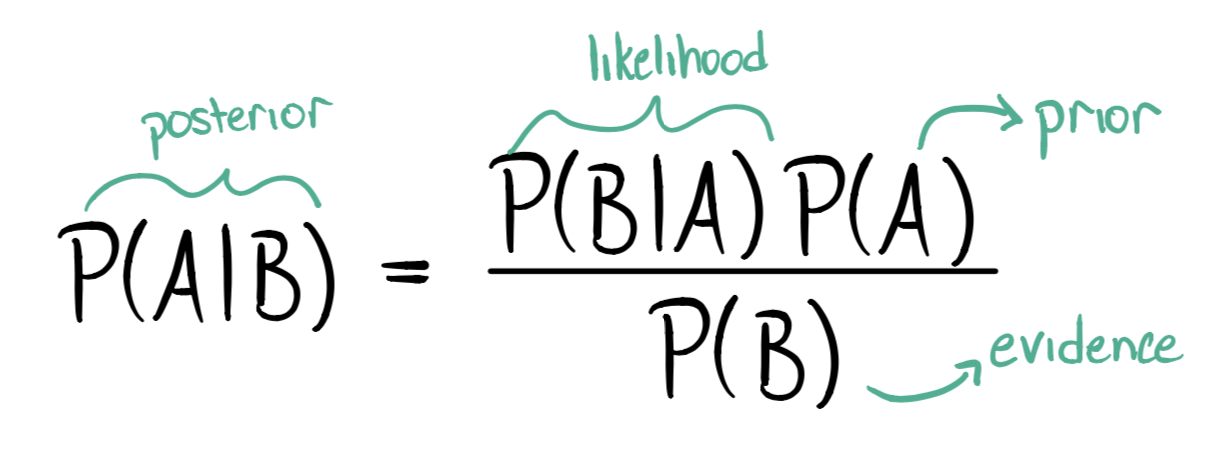
\includegraphics[scale=0.25]{bayes.png}
            \caption{Định lý ``Bayes''}
            \label{fig_bayes}
        \end{figure}
        
        \subsubsection{Khó khăn trong việc tính toán}
        Với góc nhìn này, ``posterior'' sẽ là giá trị mà chúng ta quan tâm đến, nó thể hiện mối quan hệ giữa ``prior'' của chúng ta và dữ liệu. 
        Việc tính toán ``posterior'' sẽ giúp chúng ta giải quyết các vấn đề trong thực tế.
        Theo công thức~\ref{equal_bayes}, để tính toán ``posterior'' ta cần phải có: ``prior'', ``likelihood'' và ``evidence''. Hai giá trị ở trên tử số (``prior'' và ``likelihood'') ta có thể dễ dàng xác định được trong hầu hết các trường hợp vì đó một phần là giả định của chúng ta về mô hình. Tuy nhiên, ở mẫu số ta cần tính:
        \begin{equation}
        \label{equal_evidence}
            p(b) = \int {p(b|a)p(a)\text{d}a = \mathbb{E}_a[p(b|a)]}    
        \end{equation}
        
        theo đó ta thấy được để tính được ``marginal likelihood'' thì ta cần tính biểu thức với dấu tích phân. Để tính giá trị này với dữ liệu ở chiều không gian thấp có thể không gặp nhiều khó khăn, nhưng khi tính toán ở những chiều không gian cao thì nó có thể trở thành một vấn đề nan giải. 
        Cụ thể ta thấy được rằng việc tính ``marginal likelihood'' sẽ thể hiện giá trị ``likelihood'' trung bình trên toàn bộ giá trị có thể xuất hiện của $a$, là những điều chưa chắc chắn trong mô hình, do đó $a$ ở chiều không gian càng cao thì việc tính toán càng trở nên phức tạp hơn. 

        Chúng ta cần chú ý thêm một vài khó khăn khác có thể phải đối mặt khi tính toán ``posterior'' đó là việc lấy ``tổ hợp'' khi dữ liệu là rời rạc thay vì giá trị liên tục. 
        Ở miền không gian liên tục thì ta có thể áp dụng hàm số trong lĩnh vực giải tích để tính toán, tuy nhiên trong những trường hợp mà chiều không gian của dữ liệu không liên lục, dữ liệu rời rạc thì việc tính toán sẽ còn phải xét thêm việc lấy tổ hợp dữ liệu. 

        Khi dữ liệu có số chiều lớn thì việc tính chính xác giá trị ``posterior'' trong thực tiễn thường sẽ là một việc cực kỳ khó khăn và bất khả thi và ta cần một vài kĩ thuật xấp xỉ thường được dùng để giải quyết việc tính ``posterior''. 

        \subsubsection{Bài toán Inference}
        Inference là một lớp bài toán để giải quyết vấn đề tìm hiểu về nhưng thứ mà ta biết được dựa trên những thứ mà ta đã biết. 
        Nói một cách khác thì bài toán này là tiến trình để có thể dưa ra kết luận giá trị ước lượng, hay khoảng tin cậy hoặc xấp xỉ một phân phối cho một ``biến ẩn'' (``latent variable'') thường được gọi là kết quả hay nhãn trong mẫu dữ liệu, dựa trên một vài các biến mà ta đã quan sát được thường được gọi là nguyên nhân hay dữ là dữ liệu đầu vào trong mẫu dữ liệu. 
        Ví dụ như ta có dữ liệu là hình ảnh của các đối tượng trong tự nhiên và có nhãn đi kèm mỗi ảnh, bài toán inference sẽ trả lời câu hỏi rằng nếu một tấm ảnh mới không có trước đó thì liệu ta có biết được nhãn của đối tượng trong ảnh hay không?. 

        ``Bayesian inferene'' là việc giải quyết bài toán inference dựa trên ``định lý Bayes''. Phương pháp Bayesian inference là một phương pháp trong lĩnh vực xác suất thống kê mà ở đó kiến thức biết được biết trước ``prior knowledge'' được mô hình hoá bởi một phân phối xác suất và được cập nhật mỗi khi có một quan sát mới và những thứ mà ta không chắc chắn hay không quan sát được sẽ được mô hình bởi một phân phôi xác suất khác. Một ví dụ kinh diển là về các tham số của ``Bayesian inference'', giả định rằng một mô hình mà dữ liệu $x$ được phát sinh từ một phân phối xác suất mà phân phối xác suất này được xác định bỏi các tham số $\theta$, tuy nhiên giá trị của $\theta$ thì ta chưa biết. Bên cạnh đó, ta giả định rằng, ta có một vài kiến thức được biết từ $\theta$ được gọi là ``prior knowledge'', nó có thể là phân phối xác suất $p(\theta)$. Sau đó, mỗi khi ta có một quan sát x mới, ta có thể cập nhật lại ``prior knowledge'' về tham số $\theta$ thông qua định lý Bayes theo công thức:

        trong đó 

        
        Bayesian Inference là một vấn đề thường được phải giải quyết trong các bài toán trong lĩnh vực xác suất thống kê tuy nhiên trong lĩnh vực học máy, nhiều phương pháp được xây dựng dựa trên việc giải quyết vấn đề Bayesian Inference. Ví dụ: ``Gaussian mixture models'' được dùng để giải quyêt bài toán phân lớp, hay ``Latent Dirichlet Allocation'' để giải quyết bài toán phân loại chủ đề văn vản. Và cả hai mô hình kể trên đều được xây dựng dựa trên việc giải quyết bài toán Bayes Inference.  

        % \subsubsection{Computational diffficulties}
        % Theo công thứ thì để tính toán ``posterior'' ta cần phải có: ``prior'', ``likelihood'' và ``evedience''. Hai giá trị ở trên tử số ta có thể dễ dàng ác định được trong hầu hết các trường hợp vì đó một phần là giả định của chúng ta về mô hình. Tuy nhiên, ở mẫu số ta cần tính:

        % để tính giá trị này với dữ liệu ở chiều không gian thấp có thể không gặp nhiều khó khăn, nhưng khi tính toán ở những chiều không gian cao thì nó có thể trở thành một vấn đề nan giải. Khi dữ liệu có số chiều lớn thì việc tính chính xác giá trị ``posterior'' trong thực tiễn thường sẽ là một việc cực kỳ khó khăn và bất khả thi và ta cần một vài kĩ thuật xấp xỉ thường được dùng để giải quyết việc tính ``posterior''. 

        % Chúng ta ca cần chú ý thêm một vài khó khăn khác có thể phải đối mặt khi giải quyết bài toán bayesian inference  như là việc lấy ``tổ hợp'' khi dữ liệu là rời rạc thay vì giá trị liên tục. 

        % % Bài toán bayesian inference thông thường sẽ xuất hiện trong các phương pháp học máy mà giả định rằng có một Graphical model và khi mà cho trước một vài dữ liệu mà ta có thể quan sát được và mục đích của chúng ta là muốn tái tạo lại dữ liệu ẩn của mô hình. Xét ví dụ trong phương pháp Latent Dircichlet Allocation, một phương pháp để xác định chủ đề của một đoạn văn bản. Ta được cho trước một tập ``từ điển'' với kích thước V từ và có T chủ đề có thể có, mô hình này giải định rằng
        % % \begin{itemize}
        % %     \item Với mỗi chủ đề, tồn tại một phân phối xác suất ``topic-word''  trên toàn bộ tập từ điển (giả định về prior)
        % %     \item Với mỗi đoạn văn bản, có tồn tại một phân phối xác suất ``document-topic'' trên toàn bộ tập các chủ đề (một giả định prior khác)
        % %     \item Với mỗi từ trong trong văn bản được lấy mẫu từ các phân phối giải định ở trên, cụ thể là đầu tiên chúng ta sẽ lấy mẫu một chủ đè từ phân phối xác suất ``document-topic'' của đoạn văn bản, tiếp theo, từ phân phối xác suất ``topic-word'' ta lấy mẫu một từ từ phân phối xác suất đi kèm với chủ đề được lấy mẫu ở bước trước. 
        % % \end{itemize}
        % % Tên của phương pháp này là xuất phát từ giả định Dirichlet pior của mô hình. Mục tiêu của mô hình là có thể suy diễn ``latent topic'' từ từ điển ta quan sát được cũng như là có thể phân rã chủ đề của từng đoạn văn bản. Kể cả khi nếu chúng ta không đi sâu vào chi tiết của mô hình LDA, chúng ta có thể nói một cách đại khái rằng với w là một véc-tơ các từ có trong từ điển và z là véc-tơ liên hệ với những từ đó, chúng ta muốn suy diễn được z dựa trên các quan sát từ w theo công thức bayes đó là:

        % %         $\text{có một công thức ở đây}$
 
        
        \subsubsection{Variational inference}
        Variational inference (VI) là một phương pháp thường hay được sử dụng để giải quyết bài toán ``Bayesian inference''.
        Phương pháp này sử dụng hướng tiếp cận là tìm ra xấp xỉ tốt nhất cho một phân phối xác suất bằng cách tìm ra giá trị của bộ tham số tốt nhất định nghĩa cho một phân phối khác, sao cho phân phối này sẽ ``gần'' với phân phối mà ta quan tâm. 
        
        Với phương pháp VI, đầu tiên ta sẽ tìm một phân phối xác suất có cùng ``họ'' (family) với phân phối xác suất mà ta quan tâm. 
        Một họ phân phối xác suất là tập các phân phối xác suất được định nghĩa bởi cùng một bộ tham số. 
        Ví như họ phân phối Gaussian sẽ được định nghĩa bởi $\mu$ là giá trị kỳ vọng (mean) và $\sigma$ là độ lệch chuẩn (standard deviation)
        Việc lựa chọn ``họ'' phân phối sẽ kiểm soát giữa độ phức tạp và độ chính xác của của phương pháp này. 
        Nếu ta giả định rằng dữ liệu tuân theo một phân phối đơn giản thì kết quả suy diễn được sẽ không quá chính xác nhưng có thể dễ dàng tìm được nghiệm tối ưu. Ngược lại nếu ta lựa chọn ``họ'' phân phối phức tạp thì sẽ khó tìm đươc nghiệm tối ưu nhưng kết quả suy diễn sẽ có kết quả tốt hơn. 

        Sau khi xác định được ``họ'' phân phối xác suất dùng để xấp xỉ phân phối xác suất mà chúng ta quan tâm thì việc tiếp theo là làm sao để tìm ra được xấp xỉ tốt nhất. 
        
        Giả sử rằng chúng ta cần sấp xỉ phân phối $p$ bởi một phân phối $q$ cùng thuộc họ phân phối $\mathcal{F}$.
        Chúng ta xét độ lỗi $\mathbb{E}(q,p)$ giữa hai phân phối xác suất $p$ và $q$, việc tìm ra bộ tham số tốt nhất được thể hiện bởi:
        \begin{equation}
        \label{equal_minErrorpq)}
            q^* = \text{arg}_{q\in\mathcal{F}} \text{min}\mathbb{E}(q,p)    
        \end{equation}
        

        Vậy trong bài toán variational inference thì làm sao để xác định hai phân phối xác suất có ``gần'' nhau hay không hay làm sao để xác định độ lỗi $\mathbb{E}(q,p)$. 
        Sự sai biệt Kullback-Leiber (KL) là một cách để tính mức độ lệch của một phân bố đối với một phân bố được chỉ định và thường được sử dụng để đo sự khác nhau giữa hai phân phối xác suất. 

        KL là môt thuật ngữ đến từ lĩnh lý thuyết thông tin, nó còn có tên gọi khác là entropy tương đối. Nói theo ngôn ngữ lý thuyết thông tin, nó đo lượng trung bình thông tin thêm vào nếu chúng ta mã hóa thông tin của phân bố $q$  thay cho mã hóa thông tin phân bố $p$.

        Nếu $p(x)$ và $q(x)$ là hai phân phối xác suất với $x$ là biến ngẫu nhiên bất kỳ, thì sự sai biệt KL sẽ được định nghĩa như sau:
        \begin{equation}
        \label{KLD}
            KL(q,p) = \mathbb{E}_q[\log q(x)] - \mathbb{E}_q[\log p(x)]    
        \end{equation}
        

        Sau khi xác định được một hàm lỗi để xấp xỉ phân phối xác suất mà chúng ta quan tâm $p$,  bởi phân phối $q$ thì bài toán sẽ trở thành việc tìm phân phối $q^*$ như sau:
        $$q^* = \text{arg}_{q\in\mathcal{F}} \text{min}\mathbb{E}_q[\log q(x)] - \mathbb{E}_q[\log p(x)] $$

        Việc tìm ra phân phối xác suất tốt nhất này trở thành một bài toán tìm nghiệm tối ưu do đó phương pháp này  có thể dễ dàng được áp dụng và mở rộng cho những trường hợp mà ta cần giải quyết một bài toán với quy mô dữ liệu lớn. 
        
        % \subsubsection{Kullback-Leiber Devergence}
        
            

        \subsubsection{ ``Maximum Likelihood Estimation''}
        \label{sec_mle}
        Trong lĩnh vực máy học, chúng ta sử dụng một mô hình để mô tả một tiến trình mà tổng hợp,
        phân tích tự động dữ liệu được thu thập để có thể giải quyết các vấn đề như tìm ra các đặc trưng,
        đưa ra các dự đoán dựa trên dữ liệu quan sát được.
        Xét ví dụ bài toán \textit{Hồi quy tuyến tính} (``Linear regression''),
        ta cần dự đoán giá trị $y$ dựa trên giá trị của véc-tơ $x$ theo công thức:
        \begin{equation}
        \label{equal_LR}
            y = wx + b
        \end{equation}
        Điều ta cần làm ở mô hình này là ``ước lượng'' giá trị tham số $w$ và $b$
        để mô hình có thể dự đoán giá trị $y$ một cách tốt nhất. 
        
        Với một mô hình máy học được mô tả bởi bộ tham số $\theta$, ta cần thực hiện ``ước lượng''
        bộ tham số $\theta$ sao cho mô hình có thể trả về kết quả tốt nhất. 
        Thay vì dự đoán một hàm số nào đó có khả năng ước lượng tham số tốt, ta cần một nguyên tắc để suy ra các hàm số cụ thể 
        cho các mô hình khác nhau.
        ``Maximum likelihood Estimation'' (MLE) là một công cụ phổ biến để thực hiện việc này.
        
        Xét tập dữ liệu gồm $m$ phần tử $\mathbb{X} = \{x_1,x_2,...,x_m\}$ là độc lập với nhau và được phát sinh từ một phân phối xác suất $p_{data}(x)$.
        Giả sử mô hình được mô tả bởi bộ tham số $\theta$. Khi đó, $p(x|\theta)$ là xác suất xảy ra sự kiện $x$ khi ta biết $\theta$.
        $p(x_1,x_2,...,x_m|\theta)$ chính là xác suất các sự kiện $x_1,x_2,...,x_m$ xảy ra đồng thời, xác suất đồng thời này được gọi là ``likelihood''.
        ``Likelihood'' của mô hình thể hiện khả năng mà bộ tham số của mô hình thể hiện mối quan hệ giữa dữ liệu mà ta có.
        Quá trình cực đại hóa ``likelihood'' là việc tối ưu khả năng mô hình thể hiện đúng nhất có thể mối quan hệ của dữ liệu.
        MLE là việc đi tìm bộ tham số $\theta$ sao cho likelihood là lớn nhất:
        \begin{equation}
        \label{equal_MLE}
                \theta = \max_{\theta} p(\mathbb{X};\theta)
        \end{equation} 
        
        Vì các phần tử trong $\mathbb{X}$ là độc lập và cố định, do đó công thức~\ref{equal_MLE} tương đương với:
        \begin{equation}
        \label{equal_MLE2}
            \theta = \max_{\theta} \prod_{i=1}^m p(x_i;\theta)
        \end{equation}        
        
        Bài toán MLE là quá trình tối ưu công thức~\ref{equal_MLE2}. Mà công thức này là một tích, thường thì việc tối ưu hóa một tích sẽ gặp rất nhiều khó khăn
        trong việc tính toán.
        Thay vào đó, ta tối ưu hàm logarit của ``likelihood'' bởi vì:
        \begin{itemize}
            \item logarit là một hàm đồng biến, ``likelihood'' sẽ lớn nhất khi logarit của `likelihood' là lớn nhất.
            \item logarit của một tích sẽ bằng tổng các logarit
        \end{itemize}
        Khi đó, bài toán MLE được đưa về bài toán ``Maximum log-likelihood Estimation''
        \begin{equation}
        \label{equal_loglikelihood}
            \theta = \max_{\theta} \sum_{i=1}^m \log(p(x_i;\theta))
        \end{equation}
        
        \textit{Gaussian likelihood} ám chỉ ``likelihood'' của mô hình với việc phân phối xác suất $p_{data}(x)$ thuộc ``họ'' Gaussian.
        Tương tự, các hàm likelihood khác cũng thường dùng trong các bài toán máy học là:
        \textit{Bernoulli likelihood, Multinomial likelihood}.
        
        

        
    


    \subsection{Mô hình ``Variational Auto-Encoder''} 
        \subsubsection{Mô hình xác suất}
        \textbf{\textit{Mô hình xác suất}} là một mô hình được dùng để mô tả một phân 
        phối xác suất hợp của dữ liệu bằng cách sử dụng một đồ thị để mô tả các biến 
        ngẫu nhiên tương tác với nhau trong phân phối xác suất. Ở đây 
        chúng tôi sử dụng từ ``đồ thị'' là một định nghĩa về cấu trúc 
        dữ liệu được mô tả trong lĩnh vực lý thuyết đồ thị. Đồ thị 
        bao gồm các đỉnh được kết nối trực tiếp với nhau thông qua 
        các cạnh. Vì cấu trúc của mô hình đươc mô tả bằng đồ thị cho 
        nên những mô hình này còn được gọi với một tên gọi khác là 
        ``Graphical model''. 
        Một graphical model sẽ thể hiện phân phối hợp như sau:
        $$p(x_1,x_2, .. ,x_N)$$
        trong đó $[x_1,x_2,..,x_N]$ là các đặc trưng dữ liệu, hoặc các tham số của mô hình,\dots Ví dụ như với bài toán phân loại thì một graphical model sẽ thể hiện cho phân phối $p(y,x, \theta)$ trong đó $x$ là đặc trưng đầu vào, $y$ là nhãn của dữ liệu và $\theta$ là trọng số của mô hình. 

        Graphical model cũng chính là một nhánh trong học máy, bằng cách thể hiện bài toán học máy dưới dạng một đồ thị. 
        Sự kết hợp giữa xác suất vào một mô hình học máy sẽ giúp mô hình ``giải thích'' vấn đề thực tế một cách tốt hơn. 
        Theo đó thì vấn đề cần quan tâm hoặc dữ liệu liên quan bởi các biến ngẫu nhiên. Và các biến ngẫu nhiên này chính là các đỉnh trong đồ thị và mối quan hệ giữa các đỉnh sẽ hình thành cạnh. Bằng cách thể hiện mối quan hệ giữa các biến dữ liệu bởi đồ thị ta dựa vào đó để có thể giải quyết các vấn đề mà chúng ta quan tâm. Ngoài ra bằng cách thể hiện bằng đồ thị, ta cũng thể hiện được tương quan giữa các biến dữ liệu, mà đa số các thuật toán máy học hiện nay thì tính tương quan giữa dữ liệu sẽ ảnh hưởng đến kết quả của mô hình. Dữ liệu có tính tương quan càng cao thì có thể sẽ ít đóng góp thêm ``thông tin'' cho mô hình thì có thể dẫn đến việc kết quả mô hình mang lại sẽ không cao. Do đó khi xây dựng thuật toán hay mô hình cho một vấn đề cụ thể, ta có thể áp dụng các kiến thức ta biết trước về lĩnh vực đó, về dữ liệu để có thể xác định các đặc trưng cho mô hình thông qua đồ thị. Ngoài ra việc sử dụng graphical cũng sẽ cung cấp một cái nhìn tổng quan về mô hình cũng như dữ liệu, từ đó việc phân tích, thiết kế và cài đặt cũng sẽ dễ dàng hơn.

        \subsubsection{Variational Auto-Encoder dưới góc nhìn xác suất}
        Với góc nhìn của một mô hình mạng nơ-ron thì ``Variational Auto-Encoder'' chỉ là một mạng nơ ron đơn giản với cấu trúc hai phần như mô hình ``Auto-Encoder'' tổng quát, gồm encoder và decoder. 
        Encoder được dùng để trích xuất đặc trưng ẩn từ dữ liệu, điểm khác biệt so với ``Auto-Encoder'' cơ bản là encoder của VAE sẽ là một phân phối xác suất.
        Và tương tự thì decoder sẽ là mạng nơ-ron cố gắng để tái tạo lại dữ liệu ban đầu từ đặc trưng ẩn.
        Hình \ref{fig_VAE} thể hiện kiến trúc cơ bản của mô hình variational Auto-Encoder.


        \begin{figure}
            \centering
            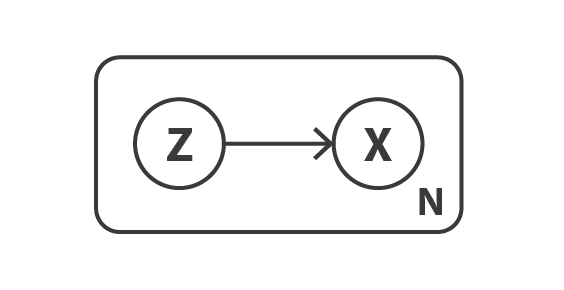
\includegraphics[scale=0.5]{dag_vae.png}
            \caption[Graphical model thể hiện cho mô hình ``Variational Auto-Encoder'']{Graphical model thể hiện cho mô hình ``Variational Auto-Encoder''. Dữ liệu quan sát được sẽ được giả định được phát sinh từ biến ẩn $z$} 
            \label{fig_dag_vae}
        \end{figure}

        Tuy nhiên để hiểu rõ hơn về nền tảng toán học cũng như xác suất trong mô hình chúng tôi sẽ trình bày mô hình VAE dưới góc độ là một mô hình xác suất.
        ``Variational Auto-enncoder'' là một mô hình đồ thị có hướng mô tả mối quan hệ giữa dữ liệu quan sát được và đặc trưng ẩn. Một đồ thị có hướng là một graphical model mà các đỉnh được kết nối với nhau có thứ tự. Có nghĩa là để có học được mẫu ở nút ``cha'' thì trước đó ta cần mô hình hoá đưọc dữ liệu ở nút con. Bên cạnh đó thì một graphical có hướng còn có tên gọi khác là ``Bayesian network''.
 
        
        Xét graphical model thể hiện cho mô hình VAE trong hình~\ref{fig_dag_vae}:
        ``Variational Auto-Encoder'' bao gồm một biến $x$ thể hiện cho dữ liệu, đây là biến dữ liệu quan sát được, và $z$ là biến ẩn thể hiện cho đặc trưng ẩn của dữ liệu. 
        Là một đồ thị có hướng do đó quá trình phát sinh dữ liệu của VAE được thực hiện qua các bước theo thứ tự như sau: 
        
        Với mỗi điểm dữ liệu: 
        \begin{itemize}
            \item Đặc trưng ẩn $z_i$ được lấy mẫu từ phân phối p(z)
            \item Điểm dữ liệu $x_i$ được lấy mẫu từ phân phối p(x|z)
        \end{itemize}

        Cụ thể, biến đặc trưng ẩn $z$ được chọn ra từ một phân phối ``prior'' $p(z)$ chính là những kiến thức ta biết trước ta biết trước hoặc là giả định của chúng ta về $z$. Điểm dữ liệu $x$ có một phân phối likelihood $p(x|z)$ thể hiện quan hệ giữa dữ liệu ta có với đặc trưng ẩn.
        Mô hình định nghĩa một phân phối hợp của dữ liệu và đặc trưng ẩn: $p(x,z)$. 
        Với quy tắc nhân trong xác suất, chúng ta có thể phân tách phân phối hợp trên thành ``prior'' và ``likelihood'' như sau: $p(x,z) = p(x|z)p(z)$. Đây chính là mục tiêu chính khi ta xét ``Variational Auto-Encoder'' dưới góc độ của xác suất.


        Mô hình này sử dụng phương pháp Variational inference được nhắc đến ở phần~\ref{chap2/subsec21} để tìm ra đặc trưng ẩn, đây cũng là lý do dẫn đến cái tên ``Variational Auto-Encoder''. Và VAE có thể được huấn luyện dựa trên các thuật toán  học dựa trên gradient truyền thống.
        
        
        Tiếp theo, ta xét đến việc suy diễn (inference) trong mô hình này. 
        Mục tiêu của việc suy diễn là tìm ra được một giá trị ``tốt'' thể hiện cho đặc trưng ẩn khi ta có các điểm dữ liệu, hay nói cách khác là ta tính ``posterior''.
        Theo công thức Bayes:
        \begin{equation}
        \label{equal_bayes1}
            p(a|b) = \frac{p(b|a)p(a)}{p(b)}
        \end{equation}
        theo như những gì đã trình bày ở những phần \ref{chap2/subsec21}, phần mẫu số 
        của công thức~\ref{equal_bayes1} được gọi là ``marginal likelihood''. 
        Và ``marginal likelihood'' sẽ không dễ dàng tính toán được một cách chính xác khi đặc trưng ẩn ở không gian có số chiều cao. 

        Do đó, phương pháp Vairational inference (VI) được áp dụng để xấp xỉ phân phối ``posterior'' $p(z|x)$ này.
        VI xấp xỉ posterior thông qua một phân phối xác suất có cùng họ phân phối $q_\lambda(z|x)$.
        Trong đó $\lambda$ thể hiện cho bộ tham số định nghĩa cho phân phối $q$, ví dụ nếu $q$ là  họ phân phối Gaussian thì $\lambda = (\mu;\sigma^2)$.
        
        Tiếp đến, ``Kullback-Leiber Devergence'' được sử dụng để xấp xỉ ``posterior'' 
        với:
        \begin{equation}
        \label{KLD1}
            \mathbb{KL}(q_\lambda(z|x) || p (z|x)) = \mathbb{E}_q[\log q_\lambda(z)] - \mathbb{E}_q[\log p(z|x)]
        \end{equation}
        trong đó các kỳ vọng đưọc lấy theo $q_\lambda(z)$.
        
        Biến đổi xác suất có điều kiện $p(z|x)$ ở công thức~\ref{KLD1}, ta có:
        \begin{equation}
        \label{KLD2}
            \mathbb{KL}(q_\lambda(z|x) || p (z|x)) =   \mathbb{E}_q[\log q_\lambda[(z|x)] - E_q[log p(x,z)] + \log p(x)
        \end{equation}
        Mục tiêu của chúng ta là tìm ra bộ tham số $\lambda$  sao cho tối thiểu được sự sai biệt trên. với $q^*$ là phân phối $q$ lý tưởng để xấp sỉ posterior thì ta có:
        \begin{equation}
        \label{equal_qlambda}
            q^*_\lambda(z|x) = \text{arg min}_\lambda KL(q_\lambda(z|x)|| p(x))
        \end{equation}        
        Tuy nhiên ta vẫn chưa có thể tính được trực tiếp bởi trong công thức thì vân còn xuất hiện $p(x)$, cho nên ``marginial likelihood'' vẫn không thể tính một cách trực tiếp.

        Vì không thể tính một cách trực tiếp ta xét một hàm số thay thế khác như sau:
        \begin{equation}
        \label{ELBO}
            ELBO(q_\lambda) = \mathbb{E}[\log p(z,x)] - \mathbb{E}[\log q_\lambda(z)]
        \end{equation}

        Biến đổi phân phối hợp $p(z,x)$ trong~\ref{ELBO}, ta lại có: 

        \begin{equation} \label{ELBO1}
            \begin{split}
                ELBO(q_\lambda) & = \mathbb{E}[\log p(z)]+ \mathbb{E}[\log p(x|z)] - \mathbb{E}[\log q_\lambda(z)]\\
                                & = \mathbb{E}[\log p(x|z)] - \mathbb{KL}( q_\lambda(z)|| p(z))
            \end{split}
        \end{equation}

        Công thức ~\ref{ELBO1} được gọi là ``evidence lower bound'' (ELBO).
        ELBO là trừ của sai biệt KL cộng với một lượng $\log p(x)$, bởi $\log p(x)$ là hằng số theo $q_\lambda(z)$.
        Bây giờ, việc cực đại ELBO sẽ tương đương với việc tối thiểu độ sai biệt KL.
        
        \label{trade_off}
        Bên cạnh đó, sau khi biến đổi mở rộng ELBO thì ta thấy rằng ELBO được tính từ 2 phần đó là kỳ vọng của likelihood và trừ KL giữa prior và phân phối sấp xỉ $q_\lambda(z)$.
        Với kỳ vọng của likelihood, nó thể hiện khả năng mô hình hoá dữ liệu còn sai biệt KL thì đảm bảo việc phân phối được xấp xỉ sẽ gần với prior của  dữ liệu.
        Đây chính là sự đánh đổi thường gặp trong những bài toán Bayesian inference, đánh đổi giữa khả năng mô hình hoá dữ liệu và việc đảm bảo phân phối được xấp sỉ hay cụ thể là đặc trưng ẩn sẽ gần với prior của chúng ta.

        % theo bất đẳng thức jensen thì Kullback-Leiber divergence luôn lớn hơn hoặc bằng không. 
        % Điều này có nghĩa rằng thay vì tối thiểu hoá KL thì ta sẽ thực hiện cực đại hoá ELBO.
        
        Sau khi nắm được lý thuyết nền tảng về xác suất của mô hình VAE, tiếp theo ta sẽ liên hệ với mạng nơ ron để thể hiện cho mô hình.
        Mục tiêu cuối cùng của chúng ta là tìm ra bộ tham số có thể xấp xỉ được posterior $ p(z|x,\lambda)$ bằng $q_\theta(z|x,\lambda) $ thông qua một mạng nơ ron thường được gọi là  ``inference network'' hay chính là encoder. Mạng này nhận đầu vào là dữ liệu $x$ và trả về kết quả là bộ tham số $\lambda$ thể hiện phân phối xác suất của đặc trưng ẩn. 
        Bên cạnh đó, sẽ có một mạng nơ ron được gọi là ``genetive network'' hay còn được biết đến là decoder thể hiện cho likelihood $p_{\phi}(x|z)$ của mô hình. 
        Tiếp theo đặc trưng ẩn sẽ được lấy mẫu từ phân phối xác suất trả ra từ encoder, đây chính là bước đầu tiên trong mô hình xác suất đã được nói ở  trên.
        Dữ liệu đầu vào của decoder là đặc trưng ẩn được lấy mẫu dựa trên phân phối của đặc trưng ẩn, và decoder sẽ cố gắng tái tạo lại dữ liệu ban đầu từ đặc trưng ẩn $z$, đây chính là bước thứ hai trong mô hình xác suất.
        
        Inference network và generative network sẽ có bộ tham số tương ứng là $\theta$ và $\phi$.
        Thông thường bộ tham số là các trọng số và bias trong một mạng nơ ron thông thường. 
        Mục tiêu của mô hình sẽ là cực đại hàm ELBO tương ứng như sau:
        \begin{equation}
        \label{ELBO2}
            ELBO(\theta,\phi) = \mathbb{E}_{q_\theta}(z|x)[\log p_\phi(x|z)] - \mathbb{KL}(q_\theta(z)||p(z))
        \end{equation}
        Để huấn luyện mô hình, ta có thể sử dụng những thuật toán học như ``gradient descent'' để có thể tìm ra bộ trọng số $\theta,\phi$.

\chapter{Mô hình ``Variational Auto-Encoder'' cho bài toán xây dựng hệ thống gợi ý}
\label{Chapter3}
\textit{Chương này chúng tôi sẽ trình bày về những tìm hiểu của chúng tôi trong việc giải quyết bài toán xây dựng hệ thống gợi ý sản phẩm. 
Đầu tiên, Chúng tôi phân tích hai loại dữ liệu phản hồi được dùng trong bài toán này từ người dùng là:
``explicit feedback'' và ``implicit feedback'' và lý do chúng tôi đặc biệt quan tâm xây dựng bài toán với dữ liệu implicit feedback.
Sau đó là việc áp dụng một mô hình Auto-encoder cơ bản để có thể xây dựng một hệ thống gợi ý sản phẩm thông qua việc trích xuất đặc trưng ẩn từ dữ liệu phản hồi và đưa ra gợi ý từ đặc trưng ẩn trên. Từ đó làm nền tảng cho việc áp dụng Variational auto-encoder để giải quyết bài toán được đặt ra. Cụ thể, mô hình Variational auto-encoder sẽ được thay đổi hàm mục tiêu để có thể phù hợp với việc gợi ý được tập sản phẩm có khả năng cao sẽ phù hợp với người dùng hơn.}


\section{Dữ liệu phản hồi của người dùng trong bài toán xây dựng hệ thống gợi ý sản phẩm}
    Như đã trình bày ở phần~\ref{Chapter1}, để xây dựng một hệ thống gợi ý 
    theo hướng tiếp cận ``Collaborative filtering'' ta chỉ cần dữ liệu là ma trận tương tác của người dùng.
    Tương tác ở đây có nghĩa là các phản hồi của người dùng dành cho sản phẩm, và các phản hồi này bao gồm hai loại:
    \begin{itemize}
        \item Phản hồi cụ thể ``explicit feedback''
        \item Phản hồi ngầm ``implicit feedback''
    \end{itemize}
    Trong phần này, chúng tôi sẽ làm rõ về tính chất của hai loại dữ liệu phản hồi cũng như ảnh hưởng của chúng đến hệ thống gợi ý.
    \subsection{Dữ liệu phản hồi cụ thể ``explicit feedback''}
    Dữ liệu phản hồi cụ thể (``explicit feedback'') được hiểu là những
    phản hồi của khách hàng về sản phẩm một cách tường minh và cụ thể, ví dụ như: số điểm đánh giá,
    bình luận, ... ``Explicit feedback'' có thể thể hiện rõ về mức độ thích/không thích của người dùng về sản phẩm;
    ví dụ người dùng có thể thể hiện sự yêu thích của họ từ 1 đến 5 sao cho một sản phẩm (một cách đánh giá thông dụng), 
    sản phẩm được đánh giá 5 sao chứng tỏ nó được thích hơn so với sản phẩm được đánh giá 4 sao. 
    Trong thực tế, dữ liệu ``explicit feedback'' thường khó để thu thập cũng như gặp trở ngại về tính tin cậy.
    Thu thập loại dữ liệu này gặp khó khăn vì không phải người dùng nào cũng sẵn sàng phản hồi về sản phẩm. 
    Sự miễn cưỡng của người dùng cũng như những tác động khi họ phản hồi có thể dẫn đến sự thiếu khách quan,
    làm sai lệch kết quả của hệ thống gợi ý. 
    Thêm nữa, vì phản hồi của người dùng thể hiện mức độ thích/không thích của người dùng, mà người dùng thì chỉ tương tác với
    một lượng sản phẩm nhỏ trên toàn hệ thống, những sản phẩm còn lại sẽ rơi vào trường hợp thiếu dữ liệu (``missing data''),
    gây khó khăn cho việc xử lí. 
    Ngày nay, số lượng sản phẩm trong hệ thống là rất lớn, ``explicit feedback'' sẽ gặp khó khăn rất lớn khi có quá nhiều trường hợp thiếu dữ liệu,
    tác động đáng kể đến hiệu quả của hệ thống. Mặt khác, ``collaborative filtering'' sẽ có cơ sở đánh giá nhóm người dùng ``tương đồng'' với nhau
    một cách khắt khe hơn, giúp các gợi ý là những sản phẩm ``tốt'' hơn, tuy nhiên đôi lúc làm cho các gợi ý không được đa dạng.

    \subsection{Dữ liệu phản hồi ngầm ``implicit feedback''}
    Dữ liệu phản hồi ngầm (``implicit feedback'') là dữ liệu được suy ra từ hành động của người dùng, nếu họ xem một bộ phim
    thì ta có thể hiểu là họ ``thích'' bộ phim đó. ``Implicit feedback'' cũng có thể được suy ra từ ``tín hiệu ngầm'' (``implicit signal''),
    xét ví dụ người dùng đánh giá một sản phẩm là 4 sao (trên thang đánh giá từ 1 đến 5 sao), từ ``tín hiệu ngầm'' dựa trên số sao họ đánh giá,
    ta có thể suy ra họ ``thích'' sản phẩm đó. 
    ``Implicit feedback'' chỉ thể hiện rõ về sự ``thích'' cũng như chỉ thể hiện một cách tương đối mức độ yêu thích của người dùng.
    Cụ thể, người dùng không xem một bộ phim không có nghĩa là họ không thích bộ phim đó, có thể là họ chưa xem hoặc không biết nó có trên hệ thống.
    Cũng như họ xem một bài hát 10 lần chứng tỏ họ thích hơn so với một bài hát họ chỉ nghe 2 lần, 
    và ``implicit feedback'' không thể thể hiện được rõ điều này.
    Trong thực tế, lượng dữ liệu phản hồi ngầm rất lớn và dễ dàng thu thập được, quá trình ``phản hồi'' của người dùng là bị động
    nên không bị ảnh hưởng bởi các yếu tố ngoại cảnh khác. 

    Ma trận tương tác của người dùng với dữ liệu phản hồi ngầm sẽ có dạng là một ma trận nhị phân, với giá trị \textbf{1} 
    thể hiện người dùng ``thích'' sản phẩm đó, giá trị \textbf{0} thể hiện hệ thống chưa có cơ sở để xác định người dùng ``thích'' sản phẩm đó.

    Với dữ liệu phản hồi ẩn, ``collaborative filtering'' sẽ xác định nhóm người dùng ``tương đồng'' với nhau rộng hơn
    do chỉ quan tâm đến các sản phẩm họ thích. Điều này sẽ giúp các gợi ý của hệ thống 
    đa dạng hơn, tuy nhiên các sản phẩm mà người dùng không thích cũng có thể sẽ được gợi ý.

    Trong giới hạn của khóa luận này, chúng tôi chỉ tìm hiểu về một hệ thống gợi ý với dữ liệu phản hồi ngầm do tính khách quan
    cũng như giải quyết được các khó khăn của ``explicit feedback''.

% \section{``Multinomial log-likelihood'' cho bài toán xây dựng hệ thống gợi ý}
\section{Xây dựng một hệ thông gợi ý sản phẩm cơ bản bằng Auto-encoder}
    Phuơng pháp xây dựng mô hình gợi ý sản phẩm mà chúng tôi tìm hiểu đó là sử đụng kiến trúc auto-encoder, một mạng nơ ron nhận input đầu vào là một phần tương tác của người dùng trong quá khứ và mô hình được huấn luyện để tái tạo lại toàn bộ tương tác của người dùng.  Mô hình này là một mạng nơ ron bao gồm hai thành phần:
    \begin{itemize}
        \item Mạng nơ-ron encoder có chức năng rút trích đặc trưng ẩn từ những tương tác của người dùng trong quá khứ
        \item Mạn nơ-ron decoder có chức năng tái tạo lại tương tác của người dùng
    \end{itemize}

    Mặc dù cách hoạt động của mô hình trong giai đoạn huấn luyện và trong giai đoạn kiểm tra có phần khác nhau, nhưng ở phần này chúng tôi chỉ trình bày cách hoạt động của mô hình trong giai đoạn huấn luyện để qua đó diễn giải kiến trúc mô hình một cách thuận tiện. Và sau đó chúng tôi sẽ trình bày cách để đưa ra gợi ý cho người dùng mới sau.

    Với tập dữ liệu được sử dụng huấn luyện gồm $U$ người dùng ${u_1,u_2, .., u_U}$ và cần xây dựng mô hình đưa ra gợi ý trong tập $I$ sản phẩm ${i_1,i_2, ..., i_I}$. Bên cạnh đó, dữ liệu tương tác của người dùng với các sản phẩm sẽ được thể hiện bởi một ma trận tương tác $X \in \mathbb{N}^{U\times I}$. Tương tác một người dùng sẽ là một véc-tơ $x_u = [x_{u1}, x_{u2}, ..., x_{uI}]^T \in \mathbb{N}^I $ với $u \in U$.
    
    Với giả định rằng việc một người dùng tương tác với các sản phẩm sẽ đến từ những đặc trưng ẩn của người dùng đó. 
    Việc trích xuất đặc trưng ẩn của ngừoi dùng dựa trên những tương tác với hệ thống trong quá khứ được hi vọng rằng những đặc đặc trưng ẩn sẽ có thể được sử dụng để thể hiện cho người dùng. 
    Sau khi có đưọc đặc trưng ẩn của người dùng thì vì dựa trên mục tiêu rằng đặc trưng sẽ thể hiện tốt được những yếu tố quyết định đến các tương tác của người dùng thì việc huấn luyện mô hình sẽ cần phải đảm bảo rằng đặc trưng ẩn có thê dùng để hình thành tương tác của người dùng. 

    
    Mục tiêu của mô hình là nhận đầu vào là tương tác của người dùng, tương tác này được chiếu vào một không gian đặc trưng có số chiều thấp hơn và sau đó lại tái tạo lại dữ liệu ban đầu với mục đích để dự đoán những sản phẩm chưa được tương tác trước đó.
    Một cách đơn giản là để huấn luyện mô hình auto-encoder là ta sẽ cố gắng tái tạo lại tương tác của người dùng để dựa vào kết quả tương tác được tái tạo để đưa ra tập sản phẩm ``tốt'' nhất mà người dùng chưa tương tác trước đó. Hoặc ta có thể xem như là một bài toán hồi quy, khi mà dữ liệu đầu vào là một con số thể hiện cho tương tác của người dùng, và mục tiêu của mô hình chính là kết quả của mô hình cũng là một véc tơ số ``gần'' với dữ liệu tương tác ban đầu.  
    Để áp dụng hướng tiếp cận cơ bản này, chúng tôi sẽ trình bày về kiến trúc của một mô hình auto-encoder để xây dựng hệ thống gợi ý cơ bản.
    Mô hình được cấu thành từ hai mạng nơ ron tách biệt được gọi là encoder và decoder. 
    Ta có thể xem rằng mạng nơ-ron encoder là một hàm phi tuyến ánh xạ dữ liệu đầu vào ở chiều không gian cao, $x_u \in R^I$ sang một không gian thấp hơn để biểu diễn cho đặc trưng ẩn $z_u \in R^k$ với $k$ là số chiều của không gian đặc trưng ẩn và thường thì $k$ sẽ rất nhỏ so với $I$. Cụ thể thì ta có:
    $$ z_u = f(W * b_1)$$
    trong đó $f(.)$ là hàm kích hoạt phi tuyến và $W,b_1$ tương ứng sẽ là trọng số và hệ số ``bias'' của encoder. 

    Sau khi có được đặc trưng ẩn, $z_u$ sẽ được lan truyền thẳng thông qua mạng nơ-ron decoder nhằm mục đích xây dựng lại tương tác ban đầu từ $z_u$
    $$x'_u = g(V \times z_u + b_2)$$
    Tương tự với encoder, $V,b_2$ sẽ tương ứng là các trọng số và ``bias'' của mạng nơ ron và g(.) chính là hàm kích hoạt của mạng nơ-ron.

    Để huấn luyện một mô hình auto-encoder để thực hiện gợi ý sản phẩm ta có thể dùng hàm chi phí sau:
    $$ \text{min}_\phi \sum_{x_u \in X}(||r - h(x_u,\theta)||^2_2)$$
    trong đó $h(x_u,\theta)$ là tương tác được tái tạo lại từ dữ liệu đầu vào cũng chính là tương tác của người dùng $u \in U$ và $x_u \in R^I$.
    $$h(x_u,\theta) = f(W \times g(V \times x_u + b_1) + b_2)$$
    với f(.) và g(.) sẽ là các hàm kích hoạt của mạng nơ-ron và $\theta = {W, V, b_1, b_2}$ với $W,V$ là trọng số tương ứng của encoder và decoder, $b_1,b_2$ tương ứng sẽ là hệ số ``bias'' của decoder và encoder.
    Với hàm chi phí này thì mô hình sẽ huấn luyện và tìm ra bộ tham số $\theta^*$ sao cho với bộ tham số này, thì mô hình sẽ có thể tự động trích xuất được những đặc trưng ẩn có thể được dùng để hình thành nên các tương tác của người dùng.

    Tuy nhiên nhiên, để có thể tính toán cũng như cập nhật trọng số cho mô hình trong tình huống mô hình được sử dụng để phát sinh gợi ý cho người dùng. 
    Cụ thể, đầu tiên, khi chúng ta huấn luyện một mạng nơ-ron phi tuyến thì tình trạng ``overfitting'' sẽ thường xảy ra, gây ảnh hưởng đến độ chính xác của mô hình. Do đó chúng ta cần phải thêm một lượng ``regular'' cho bộ tham số $\theta$.
    Thứ hai, chúng ta cần phải xét đến việc rằng dữ liệu đầu vào của chúng ta là $x_u \in R^I$ là một véc-tơ có dạng bag-of-world. 
    Có nghĩa là chỉ có phần sản phẩm là có tương tác, một người dùng chỉ tương tác một lượng ít sản phẩm chứ không phải toàn bộ.
    Do đó để những trương tác trong quá khứ của một người dùng có thể được dùng để thể hiện được đặc trưng ẩn của người đó, chúng ta chỉ cập nhật trọng số cho những nơ-ron mà có kết nối đến những sản phẩm mà người dùng đã tương tác.
    Vậy nên đê huấn luyện mô hình auto-encoder với bài toán xây dựng hệ thống gợi ý sản phẩm ta sẽ huấn luyện mô hình để tìm được bộ tham số cho mô hình, ta sẽ huấn luyện với hàm mục tiêu sau:
    $$ \text{min}_\phi \sum_{x_u \in X}(||r - h(x_u,\theta)||^2_\mathcal{O})  + \frac \lambda 2 \times (||W||^2_2 + ||V||2_2)$$
    trong đó $||.||^2_\mathcal{O}$ có nghĩa là chúng ta chỉ xét đến những tương tác xảy ra, bỏ qua đóng góp của các nơ-ron liên kết với các sản phẩm không có tương tác. 

    Với kiến trúc trên, mô hình xây dựng cho hệ thống gợi ý với số lượng sản phẩm là I và đặc trưng ẩn với số chiều là k thì số lượng tham số của mô hình sẽ là $2Ik + I + k$.
    
    Sau khi huấn luyện mô hình với hàm mục tiêu trên, ta tìm được được bô tham số $\theta^*$, thì để dự đoán số điểm tương tác của người dùng u với sản phẩm i cụ thể sẽ là: 
    $$\widehat{x}_{ui} = h(x_{ui},\theta^*)$$

    Đây chính là kiến trúc cơ bản nhất khi ta sử dụng mô hình auto-encoder để xây dựng một thống gợi ý sản phẩm.
    


   



    \subsection{Tăng khả năng phát sinh gợi ý cho người dùng bằng kỹ thuật ``drop-out''}
    Như đã thảo luận ở phần trên, thì chúng ta đã xây dựng một kiến trúc cơ bản nhất trong việc xây dựng một hệ thống gợi ý sản phẩm dựa trên mô hình auto-encoder.
    Tuy nhiên, mô hình trên vẫn còn nhiều hạn chế sau: 
    \begin{itemize}
        \item  Mặc dù, để phù hợp với bài toán gợi ý sản phẩm thì chúng ta chỉ tập nhật trọng số có liên kết với các phần tử là tương tác của người trong tập $\mathcal{O}$, là tập tương tác của người dùng, nhưng thưc tế thì mô hình vẫn đang làm tác vụ là tái tạo lại tương tác của người dùng từ đặc trưng ẩn phát sinh từ tương tác của người dùng. 
        \item Một hạn chế khác đó là tính trạng overfiting, khi huấn luyện mạng nơ-ron. Với việc thêm `regular' để huấn luyện nhưng với dữ liệu thưa thì, regular sẽ không thực sự hiệu quả.
    \end{itemize}
    Một phương pháp mà chúng tôi sử dụng để có thể giải quyết những vấn đề trên đó là chúng tôi che đi một số tương tác trước khi dữ liệu được truyền thẳng qua mạng encoder. 
    Cụ thể thì chúng tôi áp dụng dropout cho véc-tở đầu vào, droput là một phương pháp ``regularization'' thường được áp dụng khi huấn luyện các mạng học sâu. 
    Dropout sẽ ép mạng nơ-ron tìm ra được những đặc trưng quan trọng hơn, hay là tìm ra những sản phẩm ảnh hưởng lớn đến đặc trưng ẩn của người dùng. 
    
    Với việc sử dụng thêm nhiễu vào dữ liệu tương tác ban đầu của người dùng sẽ mang lại cho mô hình auto-encoder phù hợp hơn và hiệu quả hơn khi huấn luyện với dữ liệu tương tác của người dùng.
    Điều đầu tiên mang lại cho mô hình khi sử dụng một tầng ``dropout'' đó là mô hình lúc này ngoài việc trọng số được cập nhật để có thể tái tạo lại dữ liệu của ngừoi dùng mà khi này, trong tương tác của người dùng đã thực sự bị che mất một phần vậy nên cả quá trình huấn luyện mô hình cũng sẽ phải học để có thể dự đoán những trương tác bị che trong dữ liệu. Nói cách khác đó là sau khi thực hiện thêm nhiễu, thì mô hình sẽ thực sự là dự đoán những tương tác bị che từ những tương tác có trước đó trong lịch sử của người dùng thay vì chỉ để tái tạo lại tương tác của người dùng trước đó.

    Bên cạnh đó, drop out là một cách hiệu quả để ngăn tình trạng ``overfitting'' hiệu quả.

    Đây cũng chính kiến trúc của một biến thể của auto-encoder đó là denosing auto-encoder đã được trình bày trong phần 2.1.3.
    

    

\section{Áp dụng mô hình ``Variational Auto-encoder'' cho bài toán gợi ý sản phẩm}
    Trong lĩnh vực trí tuệ nhân tạo thì dữ liệu đóng vài trò cực kỳ quan trọng.
    Đặc biệt là lĩnh vực máy học, thì hiểu được dữ liệu sẽ góp phần không ít đến việc xây dựng một mô hình hiệu quả. 
    Do đó, để có thể tận dụng được tính chất của dữ liệu trong bài toán xây dựng gợi ý sản phẩm đó là thưa, có nghĩa là người dùng trong thực tế sẽ chỉ tương tác với một lượng nhỏ số lượng sản phẩm.
    Với đặc điểm này, cũng chính là lý do mà tác giả trong bài báo mà chúng tôi tìm hiểu đã đề xuất việc sử dụng mô hình variational auto-encoder, một biến thể đặc biệt của auto-encoder cơ bản để xây dựng hệ thống gợi ý sản phẩm.

    Ở phần này chúng tôi sẽ trình bày về kiến trúc mô hình đã tìm hiểu cho bài toán gợi ý sản phẩm trong bài báo cũng như là những đề xuất cải thiện cho mô hình VAEs trong tác vụ gợi ý sản phẩm cho người dùng. 

    \subsection{Mô hình variational autoencoder cho bài toán gợi ý sản phẩm}
    Dữ liệu lương tác trong hệ thống gợi ý sản phẩm thường là dữ liệu thưa, có nghĩa là các phần tử trong véc-tơ input đầu vào sẽ đa phần sẽ mang giá trị 0. 
    Ngoài ra, mục tiêu của một hệ thống gợi ý sản phẩm chính là việc tăng thêm số lượng tương tác của người dùng lên hệ thống, đặc biệt là khi người dùng chưa tương tác nhiều.
    Do đó, trong trường hợp này, nếu áp dụng những phương pháp dựa trên mạng nơ-ron thông thường sẽ dễ dẫn đến tình trạng ``overfiting'' khi mà dữ liệu đầu vào ít nên mô hình không học được.
    
    Dựa vào hạn chế này, bài báo đã đề xuất việc sử dụng mô hình variation auto-encoder. 
    Tuy là một mô hình mạng nơ-ron nhưng với nền tảng xác suất, cụ thể là phương pháp variational inference, là một phương pháp suy diễn dữ liệu trong lĩnh vực xác suất thống kê.
    Như đã trình bày ở phần 2.2, đây là một biến thể đặc biệt của auto-encoder cơ bản, với việc đặc trưng ẩn được rút trích là một phân phôi xác suất, mô hình đã mang lại ý nghĩa xác suất cho đặc trưng ẩn.
    Nói cách khác, đặc trưng giờ đây k chỉ thể hiện cho tương tác của người dùng, ngoài ra, là một phân phối xác suất thì đặc trưng ẩn sẽ thể hiện đưọc nhiều điều hơn về tương tác của người dùng.


    Nếu ta sử dụng tất cả tương tác của người dùng để trích xuất được những đặc trưng ẩn, thì có thể sẽ bị ảnh hưởng bởi nhiễu, hay có thể sẽ có những sản phẩm ``không quan trọng'' trong việc thê hiện đặc trưng của người dùng nên đặc trưng ẩn sẽ mang theo tất cả các thông tin đó, điều này có thể dẫn đến việc overfiting khi dữ liệu thưa, hay tương tác của người dùng còn ít.
    Những sản phẩm ``không quan trọng'' có thể xen là những sản phẩm mà không xuất hiện theo mẫu tương tác chung giữa các người dùng, những sản phẩm có thể sẽ là những sản phẩm đặc biệt của những người dùng có sở thích ``khác biệt'' so với những người dùng còn lại. 
    Vì theo ý tưởng của collaborative, là hướng tiếp cận mà nhóm tìm hiểu để xây dựng hệ thống gợi ý, thì việc đưa ra gợi ý cho một người dùng sẽ dựa trên việc mô hình tìm ra được những mẫu tương tác chung giữa các người dùng và mẫu tương tác chung này sẽ được thể hiện thông qua đặc trưng ẩn.
    Ngược lại, nếu từ tương tác của người, ta phát sinh một phân bố để thể hiện cho đặc trưng ẩn, thì khi sử dụng đặc trưng ẩn để đưa ra gợi ý, thì điểm ``tốt nhất'' trong phân bố, cụ thể ở bài báo được đề xuất là giá trị trung bình của phân bố sẽ được lấy để đưa ra gợi ý.
    Vì là một phân bố, những sản phẩm ``ko quan trọng'' sẽ ít đóng góp ít hơn ở điểm trung bình. Vì điểm trung bình sẽ là điểm có phân phối xác suất cao nhất, có nghĩa là tập sản phẩm ít xuất hiện trong xu hướng tương tác chung của các người dùng trong hệ thống sẽ đóng góp ít hơn ở điểm trung bình. 

    

    \subsection{Thay đổi hàm lỗi để phù hợp hơn cho bài toán gợi ý sản phẩm}
        \subsubsection{Multinomial likelihood}
        \subsubsection{Beta variational auto-encoder}
    


\chapter{Thí nghiệm}
\label{Chapter4}
\graphicspath{{Chapter4/Chapter4Figs}}
\textit{Trong chương này, chúng tôi trình bày các kết quả thí nghiệm nhằm đánh giá những nội dung trình bày ở chương \ref{Chapter3}. Bộ dữ liệu được dùng để tiến hành các thí nghiệm là bộ MovieLens-20M \cite{Ml20M} và Million Song Dataset \cite{MSD}; bên cạnh đó, độ đo được sử dụng để đánh giá khả năng đưa ra gợi ý của mô hình là Normalized Discounted Cumulative Gain (NDCG) và  Recall. Kết quả thí nghiệm cho thấy mô hình do chúng tôi cài đặt đạt được kết quả xấp xỉ so với kết quả được công bố trong bài báo \cite{mvae}. Bên cạnh đó, các kết quả thí nghiệm cũng chứng tỏ mô hình "Variational Auto-Encoder" có khả đưa ra các gợi ý sản phẩm phù hợp hơn so với mô hình "Auto-Encoder" cơ bản, đặc biệt là trong trường hợp dữ liệu tương tác của người dùng thưa. Ngoài ra, các kết quả thí nghiệm cũng cho thấy việc thay đổi hàm mục tiêu trong quá trình huấn luyện giúp mô hình đưa ra kết quả tốt hơn cho bài toán gợi ý sản phẩm.}


\section{Tập dữ liệu sử dụng}
\label{chap4sec1}
Chúng tôi tiến hành thí nghiệm trên các tập dữ liệu vừa và lớn ở các lĩnh vực khác nhau là MovieLens-20M \cite{Ml20M} 
và Million Song Dataset (MSD) \cite{MSD}; đây là các tập dữ liệu thường được dùng cho bài toán xây dựng hệ thống gợi ý
với hướng tiếp cận ``Collaborative Filtering''. 
\begin{itemize}
    \item Tập dữ liệu MovieLens-20M bao gồm dữ liệu đánh giá của 138,000 người dùng với khoảng 27,000 bộ phim,
    với 20 triệu đánh giá.
    \item Tập dữ liệu Million Song Dataset bao gồm dữ liệu tương tác (số lượt nghe) của khoảng 1 triệu người dùng và hơn 300,000 bài hát, với hơn 48 triệu tương tác.
\end{itemize}

Để có thể đánh giá kết quả đạt được so với kết quả trong bài báo \cite{mvae} một cách tốt nhất,
chúng tôi thực hiện các bước tiền xử lí được các tác giả mô tả trong bài báo \cite{mvae}.
\begin{itemize}
    \item Tập dữ liệu MovieLens-20M: chúng tôi giữ lại những người dùng đã đánh giá ít nhất 5 bộ phim trở lên. 
    \item Tập dữ liệu Million Song Dataset: chúng tôi chỉ giữ lại những bài hát được nghe bởi ít nhất 200 người dùng, và những người dùng nghe ít nhất 20 bài hát trong số còn lại.
\end{itemize}

Sau khi lọc dữ liệu theo điều kiện đã nói, số lượng người dùng, số lượng sản phẩm, số lượng tương tác, tỉ lệ tương tác giữa người dùng và sản phẩm được mô tả trong bảng~\ref{table_dataset}.
\begin{table}[]
\centering
    \begin{tabular}{|l|c|c|}
    \hline
                                                & \textbf{MovieLens} & \textbf{MSD}    \\ \hline
    \textbf{Số lượng người dùng}                  & 136,677            & 571,355         \\ \hline
    \textbf{Số lượng sản phẩm}                    & 20,108             & 41,140          \\ \hline
    \textbf{Số lượng tương tác}                   & 10.0M              & 33.6M           \\ \hline
    \textbf{\% tương tác}                         & 0.36               & 0.14            \\ \hline
    \textbf{Số người dùng trong tập ``held-out``} & \textbf{10,000}    & \textbf{50,000} \\ \hline
    \end{tabular}
   
    \caption{Thống kê số lượng người dùng, số lượng sản phẩm, số lượng tương tác trong các tập dữ liệu}
    \label{table_dataset}    
\end{table}


Chúng tôi tiến hành ``chuẩn hóa'' dữ liệu về dạng ``implicit feedback''. Đối với tập dữ liệu MovieLens, chúng tôi 
chúng tôi chuyển dữ liệu thành dạng ma trận tương tác nhị phân, với các đánh giá của người dùng từ 4 trở lên (nghĩa là người dùng thích bộ phim đó) mang giá trị 1 trong ma trận nhị phân.
Với tập dữ liệu MSD, chúng tôi chuyển các giá trị tương tác của người dùng (số lượt nghe) thành giá trị nhị phân, có nghĩa là nếu người dùng đã nghe bài hát đó thì sẽ mang giá trị 1 trong ma trận nhị phân.

Với mỗi tập dữ liệu, chúng tôi lần lượt lấy ra một số lượng người dùng bằng nhau cho tập đánh giá (validation) và tập kiểm tra (testing), gọi chung đây là các tập ``held-out''. 
Số lượng người dùng cho mỗi tập ``held-out'' được thống kê lại trong \ref{table_dataset}.
Phần còn lại sẽ là tập dữ liệu huấn luyện (training).
Ngoài ra mỗi tập trên đều sẽ được chia làm 2 phần với mục đích tính toán độ đo để đánh giá mô hình.
Cụ thể thì mỗi tập sẽ được chia thành hai phần ``fold-in'' và ``fold-out''.
``fold-in'' là phần sẽ là đầu vào của mô hình thể hiện cho dữ liệu tương tác trong qua khứ của người dùng. 
Phần còn lại dùng để đánh giá kết quả của mô hình.
Tỉ lệ giữa ``fold-in'' và ``fold-out'' mặc định là 8:2 khi đánh giá mô hình.


\section{Các thiết lập thí nghiệm}
\label{setup_experiment}

Để đánh giá khả năng tổng quát hóa của mô hình, chúng tôi chia dữ liệu thành 3 phần như đã trình bày trong phần~\ref{chap4sec1}, bao gồm các tập huấn luyện, đánh giá, kiểm tra. Với số người dùng của các tập ``held-out'' (tập dữ liệu đánh giá và kiểm tra) lần lượt là 10,000 và 50,000 cho hai bộ dữ liệu MovieLens và MSD.

Để huấn luyện mô hình, chúng tôi sử dụng toàn bộ dữ liệu tương tác của người dùng trong tập huấn luyện. Để đánh giá mô hình, chúng tôi dùng phần ``fold-in'' trong tập ``held-out'' làm đầu vào của mô hình. Sau đó đánh giá các sản phẩm được dự đoán bởi mô hình dựa trên tập ``fold-out'' với hai độ đo ``Normalized Discounted Cumulative Gain'' (NDCG) và ``Recall'' (chi tiết về độ đo đánh giá hệ thống gợi ý sản phẩm được trình bày trong phụ lục~\ref{chap_metrics}).

Chúng tôi sử dụng một kiến trúc giống nhau cho hai mô hình ``Auto-encoder'' và ``Variational Auto-encoder'' (VAE). Với ``encoder'' và ``decoder'' là mạng nơ-ron nhiều lớp (``Multi-layer Perceptron'' hay MLP) có kiến trúc đối xứng nhau, kích thước véc-tơ biểu diễn ẩn của mô hình là 200. Kiến trúc của các mô hình trên với MLP có 1 tầng ẩn kích thước 600 có thể mô tả ngắn gọn là $[ I \to 600 \to 200 \to 600 \to I ]$, với I là số lượng sản phẩm. Áp dụng hàm kích hoạt phi tuyến là \textit{tanh} giữa các lớp, tuy nhiên, do đầu ra của ``encoder'' trong mô hình VAE là một phân phối xác suất, do đó chúng tôi không áp dụng hàm kích hoạt tầng đó.

Ngoài ra, như đã trình bày ở phần~\ref{DAE_recsys}, chúng tôi áp dụng kỹ thuật ``dropout'' cho véc-tơ đầu vào để tăng khả năng sinh ra gợi ý của mô hình cũng như tránh tình trạng ``overfitting''.

Như đề xuất của tác giả Liang trong bài báo \cite{mvae}, chúng tôi sử dụng ``Multinomal log-likelihood'' làm hàm tính độ lỗi cho cả hai mô hình. Chúng tôi gọi mô hình ``Variational Auto-encoder'' với hàm lỗi này là Mult-VAE, mô hình ``Auto-encoder'' với hàm lỗi này và phần ``dropout'' là Mult-DAE.

Chúng tôi điều chỉnh siêu tham số $\beta$ của mô hình Mult-VAE với 200,000 bước cập nhật theo phương pháp ``KL-annealing'' được trình bày ở phần~\ref{subsubsecELBO}. Và áp dụng một lượng ``weight-decay'' 0.01 cho Mult-DAE. 

Chúng tôi lần lượt huấn luyện hai mô hình Mult-VAE và Mult-DAE bằng thuật toán Adam \cite{Goodfellow-et-al-2016-Book} với hệ số học (``learning rate'') là \textit{0.001} trên các tập dữ liệu MovieLens \cite{Ml20M} với 200 ``epoch'' và Million Song Dataset \cite{MSD} với 100 ``epoch'' (mỗi ``epoch'' là một lần mô hình duyệt qua hết dữ liệu huấn luyện).


\section{Các kết quả thí nghiệm}
    \subsection{Kết quả cài đặt của khóa luận so với bài báo}
    \label{experiment1}
    Trong phần này, chúng tôi sẽ trình bày kết quả của mô hình mà chúng tôi cài đặt. 
    Cụ thể, chúng tôi so sánh kết quả mô hình Mult-VAE và Mult-DAE chúng tôi cài đặt so với kết quả trong bài báo.
    Các mô hình được đánh giá trên tập kiểm tra gồm 10,000 người dùng trong tập dữ liệu MovieLens và 50,000 người dùng trong tập Million Song Dataset.
    Chúng tôi dùng các độ đo giống với mô tả trong bài báo là:
    \begin{itemize}
        \item NDCG@100: độ đo NDCG trên tối đa 100 sản phẩm được mô hình xếp hạng cao nhất.
        \item Recall@50: độ đo Recall trên tối đa 50 sản phẩm được mô hình xếp hạng cao nhất.
        \item Recall@20: độ đo Recall trên tối đa 20 sản phẩm được mô hình xếp hạng cao nhất.
    \end{itemize}

    Từ kết quả trên bảng~\ref{table:ML20MResult}, ở tập dữ liệu MovieLens, cả hai mô hình chúng tôi cài đặt đều đạt được kết quả tương đồng so với kết quả trong bài báo \cite{mvae}.
    \begin{table}[]
        \centering
        \begin{tabular}{|l|c|c|c|}
            \hline
                            & \textbf{Recall@20} & \textbf{Recall@50} & \textbf{NDCG@100} \\ \hline
            \textbf{Mult-VAE} & 0.395              & 0.537              & 0.429             \\ \hline
            \textbf{\begin{tabular}[c]{@{}l@{}}Mult-VAE\\ (cài đặt của tác giả)\end{tabular}} & 0.395 & 0.537 & 0.426 \\ \hline
            \textbf{Mult-DAE} & 0.398              & 0.535              & 0.423             \\ \hline
            \textbf{\begin{tabular}[c]{@{}l@{}}Mult-DAE\\ (cài đặt của tác giả)\end{tabular}}  & 0.387 & 0.524 & 0.419 \\ \hline
            \end{tabular}
        \caption[Kết quả cài đặt trên tập MovieLens]{Kết quả cài đặt trên tập MovieLens so với kết quả trong bài báo \cite{mvae}}
        \label{table:ML20MResult}
        \end{table}

        
    Với các kết quả tập dữ liệu MSD được thể hiện trong bảng~\ref{table:MSDResult}, cả hai mô hình chúng tôi cài đặt cho kết quả có sai lệch so với kết quả trong bài báo.
    Nhìn chung, kết quả của Mult-VAE và Mult-DAE ở cả 3 độ đo đều tương quan so với kết quả của bài báo.
    \begin{table}[]
        \centering
        \begin{tabular}{|l|c|c|c|}
        \hline
                            & \textbf{Recall@20} & \textbf{Recall@50} & \textbf{NDCG@100} \\ \hline
        \textbf{Mult-VAE} & 0.257              & 0.353              & 0.308             \\ \hline
        \textbf{\begin{tabular}[c]{@{}l@{}}Mult-VAE\\ (cài đặt của tác giả)\end{tabular}} & 0.266 & 0.364 & 0.316 \\ \hline
        \textbf{Mult-DAE} & 0.256              & 0.351              & 0.306             \\ \hline
        \textbf{\begin{tabular}[c]{@{}l@{}}Mult-DAE\\ (cài đặt của tác giả)\end{tabular}}  & 0.266 & 0.363 & 0.313 \\ \hline
        \end{tabular}

        \caption[Kết quả cài đặt trên tập MSD]{Kết quả cài đặt trên tập MSD so với kết quả trong bài báo \cite{mvae}}
        \label{table:MSDResult}
    \end{table}

    Với mô hình Mult-VAE, cài đặt của tác giả Lobel và các cộng sự trong bài báo ``RACT: Towards amortized ranking-critical trainning for collaborative filtering'' \cite{ract}, mô hình của tác giả cài đặt cũng cho kết quả tương đồng với mô hình chúng tôi cài đặt, với sai số nhỏ.
    Theo đó, kết quả trên tập dữ liệu MovieLens tương đồng với bài báo gốc \cite{mvae} và kết quả trên tập dữ liệu MSD (được trình bày trong bảng~\ref{table_compareMSD}) thấp hơn bài báo gốc, tuy nhiên sai số không quá lớn. 

    
    Qua các kết quả trên, chúng tôi rút ra nhận xét như sau. Mult-VAE cho kết quả tốt hơn Mult-DAE ở cả 3 độ đo trên tập dữ liệu MovieLens.
    Với tập dữ liệu có kích thước lớn hơn là MSD, cả Mult-VAE và Mult-DAE đều cho kết quả khá gần nhau ở cả 3 độ đo, tương đồng với kết quả của hai mô hình này trong bài báo gốc \cite{mvae}.
    

    \begin{table}[]
        \centering
        \begin{tabular}{|l|c|c|c|}
        \hline
                                                                                                & \textbf{Recall@20} & \textbf{Recall@50} & \textbf{NDCG@100} \\ \hline
        \textbf{Mult-VAE}                                                                       & 0.257              & 0.353              & 0.308             \\ \hline
        \textbf{\begin{tabular}[c]{@{}l@{}}Mult-VAE\\ (cài đặt của tác giả Lobel)\end{tabular}} & 0.260              & 0.356              & 0.310             \\ \hline
        \textbf{\begin{tabular}[c]{@{}l@{}}Mult-VAE\\ (cài đặt của tác giả Liang)\end{tabular}} & 0.266              & 0.364              & 0.316             \\ \hline
        \end{tabular}
        \caption[]{Kết quả cài đặt của khoá luận so với kết quả cài đặt trong bài báo của tác giả Lobel \cite{ract} và  bài báo của tác giả Liang \cite{mvae} trên tập dữ liệu MSD}
        \label{table_compareMSD}
        \end{table}
    \subsection{Phân tích ``Multinomial Likelihood''}

    Ở phần này, chúng tôi sẽ trình bày thí nghiệm để kiểm chứng hàm lỗi Multinomial log-likelihood so với các hàm lỗi thường được dùng khác.
    Cụ thể chúng tôi sẽ so sánh Multinomial log-likelihood so với Gaussian log-likelihood và Logistic log-likelihood. 


    Hàm ``Multinomaial log-likelihood'' như đã được trình bày ở phần \ref{mulll} sẽ giả định dữ liệu ban đầu sẽ được phát sinh bởi một phân phối đa thức (``Multinomial Distribution'').
    Và kết quả trả về của mô hình Mult-VAE là một véc-tơ thể hiện xác suất được chọn của từng sản phẩm trong hệ thống (véc-tơ này có tổng bằng 1).
    
    Về Gaussian log-likelihood, cũng chính là độ lỗi ``Mean Square Error'', là một độ lỗi thường gặp trong những bài toán hồi quy (regression). 
    Với độ lỗi này thì dữ liệu tương tác của người dùng được giả định sẽ tuân theo phân phối Gaussian. 
    Theo đó, chúng tôi dựa vào bài báo \cite{yifan_cf} của tác giả Yifan Hu, đã áp dụng Gaussian log-likelihood cho bài toán gợi ý sản phẩm với dữ liệu ``implicit feedback''. 
    Theo bài báo thì Gaussian log-likelihood cho người dùng $u$ sẽ là:
    \begin{equation}
        \log p_\theta(x_u|z_u) = -\sum_i \frac{c_{ui}}{2}(x_{ui} - f_{ui})^2
    \end{equation}
    trong đó, $c_{ui}$ là hệ số ``confidence'' của tương tác được thực hiện bởi người dùng $u$ với sản phẩm $i$ và $f_{ui}$ là kết quả tái tạo lại tương tác của người dùng $u$ với sản phẩm $i$.
    Hệ số ``confidence'' $c_{ui}$ kiểm soát sự ảnh hưởng giữa những sản phẩm được tương tác với những sản phẩm không được tương tác.
    Cụ thể, những sản phẩm được tương tác sẽ có giá trị hệ số ``confidence'' cao hơn so với những sản phẩm không tương tác.
    Có nghĩa là $c_{1}  > c_0$, với $c_1,c_0$ lần lượt là hệ số ``confidence'' của sản phẩm được tương và sản phẩm không được tương tác. 
    
    Bên cạnh đó, Logistic log-likelihood, hay còn được biết đến là độ lỗi ``Binary cross entropy'', là một độ lỗi thường được dùng trong những bài toán phân loại (classification).
    Về lý thuyết xác suất, sử dụng mô hình này ta sẽ giả định rằng dữ liệu của chúng ta sẽ được phát sinh từ một phân phối Bernoulli. 
    Với việc sử dụng, Logistic log-likelihood thì bài toán xây dựng hệ thống gợi ý sản phẩm hay cụ thể việc xác định tương tác của một người dùng với một sản phẩm sẽ được xem như bài toán phân loại 2 lớp. 
    Logistic log-likelihood của người dùng u sẽ được tính như sau:
    \begin{equation}
        \log p_\theta(x_u|z_u) = -\sum_i x_{ui}\log \sigma(f_{xui}) + (1-x_{ui})\log(1 - \sigma(f_{ui}))
    \end{equation}
    Trong đó $\sigma(x) = \frac{1}{1+\exp (-x)}$ là hàm logistic và  $f_{ui}$ là kết quả tái tạo lại tương tác của người dùng $u$ với sản phẩm $i$.
    Để thể hiện sự hiệu quả của multinomial log-likelihood so với hai hàm lỗi còn lại trong bài toán gợi ý sản phẩm với sản phầm phản hồi ngầm, chúng tôi lần lượng thực hiện huấn luyện mô hình với các độ lỗi trên và ghi lại kết quả tốt nhất. 
    Trong thí nghiệm này việc huấn luyện mô hình chỉ thay đổi độ lỗi và các thiết lập khác sẽ được giữ nguyên.
    Cụ thể, chúng tôi tiến hành thay đổi hàm lỗi ``Multinomial log-likelihood'' thành các hàm lỗi ``Gaussian likelihood'' và ``Logistic log-likelihood'' trên hai mô hình ``Variational Auto-encoder'' và ``Auto-encoder'' với các thiết lập giống phần~\ref{setup_experiment}.
    Và chúng tôi thực hiện ``fine-tune'' siêu tham số tách biệt giữa các độ lỗi với nhau.
    Vì tính chất của ``Multinomial log-likelihood'' phục vụ mục đích xếp hạng các sản phẩm ``phù hợp'' với người dùng, do đó chúng tôi dùng độ đo Normalized Discounted Cumulative Gain (NDCG) để đánh giá chất lượng xếp hạng của mô hình. 
    
    Kết quả thực nghiệm được ghi nhận lại ở bảng~\ref{table:comparell} thể hiện độ đo NDCG@100 với các hàm lỗi và mô hình tương ứng. 
    Từ kết quả cho ta thấy ảnh hưởng của ``Multinomial log-likelihood'' lên chất lượng xếp hạng của mô hình (đánh giá thông qua độ đo NDCG@100). 
    Điều này chứng tỏ được rằng việc lựa chọn hàm lỗi thực sự phụ thuộc vào dữ liệu của mô hình. 
    Và đối với bài toán gợi ý sản phẩm, cụ thể là với dữ liệu phản hồi ngầm thì multinomial log-likelihood mang lại kết quả ấn tượng. 
    Từ đó cho thấy ``Multinomial log-likelihood'' là một hàm lỗi phù hợp với hệ thống gợi ý, khi chúng ta muốn ``xếp hạng'' các sản phẩm, từ đó đưa ra các gợi ý tốt nhất cho người dùng.            

    \begin{table}[]
    \centering
        \begin{tabular}{|c|c|c|c|}
        \hline
                        & \textbf{Multinomial}                  & \textbf{Gaussian}            & \textbf{Logistics}           \\ \hline
        \textbf{VAE} &  \textbf{0.429} & 0.422 &  0.419 \\ \hline
        \textbf{DAE}  & \textbf{0.423}                        & 0.409                        & 0.412                        \\ \hline
        \end{tabular}
    
    \caption[]{Độ đo NDCG@100 trên các mô hình VAE và DAE với các hàm lỗi khác nhau trên tập dữ liệu MovieLens}
    \label{table:comparell}
    \end{table}



    \subsection{``Variational Auto-encoder'' và ``Auto-encoder'' đối với trường hợp dữ liệu thưa}
    Trong phần này, mục tiêu của  chúng tôi là kiểm chứng về sự phù hợp của ``Variational Auto-encoder'' so với ``Auto-encoder'', cụ thể là so sánh Mult-VAE và Mult-DAE.
    Theo góc nhìn khác thì ta có thể xem như đây là thí nghiệm so sánh giữa phương pháp ``Bayesian inference'' cho đặc trưng ẩn là một phân bố so với hướng tiếp cận xấp xỉ đặc trưng ẩn là một điểm xác định.

    Như đã trình bày ở mục \ref{why_vae}, thì mô hình Mult-VAE được xây dựng dựa trên các giả định của chúng tôi về dữ liệu, cụ thể là khi dữ liệu thưa.
    Do đó chúng tôi sẽ đánh giá hai mô hình Mult-VAE với tình trạng dữ liệu thưa.

    Theo thí nghiệm ở mục \ref{experiment1} thì ta có thể thấy được ở tập MovieLens thì cách biệt giữa Mult-VAE và Mult-DAE là lớn hơn so với tập MSD.
    Để kiểm chứng hiệu quả của Mult-VAE tốt hơn Mult-DAE ở điều kiện dữ liệu thưa, ở thí nghiệm này, cụ thể thì trong tập kiểm tra chúng tôi sẽ lần lượt thí hiện giảm số lượng tương tác người dùng trong tập ``fold-in'' (ở đánh giá trước các đánh giá dựa trên tập ``fold-in'' gồm 80\% tương tác của người dùng). Và đánh giá kết quả của mô hình dựa trên số lượng tương tác còn lại.
    
    \begin{figure}
        \centering
        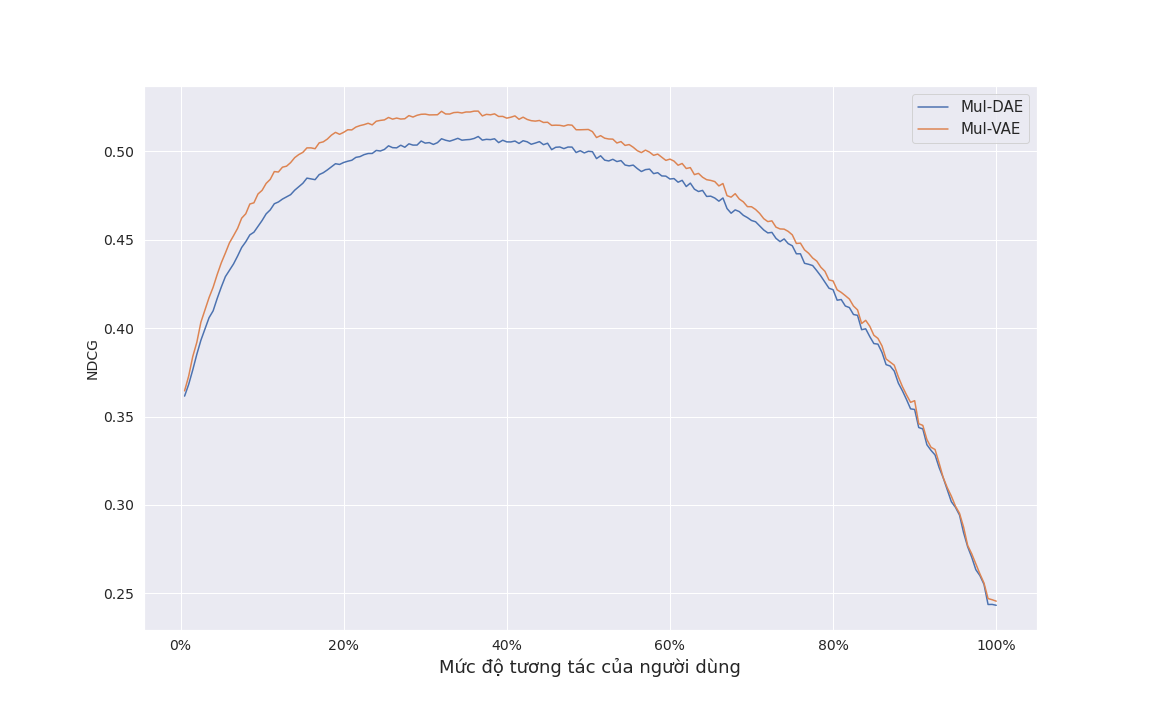
\includegraphics[width=1\textwidth]{vae_dae_ml.png}
        \caption{So sánh Mult-VAE và Mult-DAE ở các mức độ tương tác khác nhau trên tập kiểm tra trên tập MovieLens}
        \label{fig_vae_dae_ml}
    \end{figure}
    \begin{figure}
        \centering
        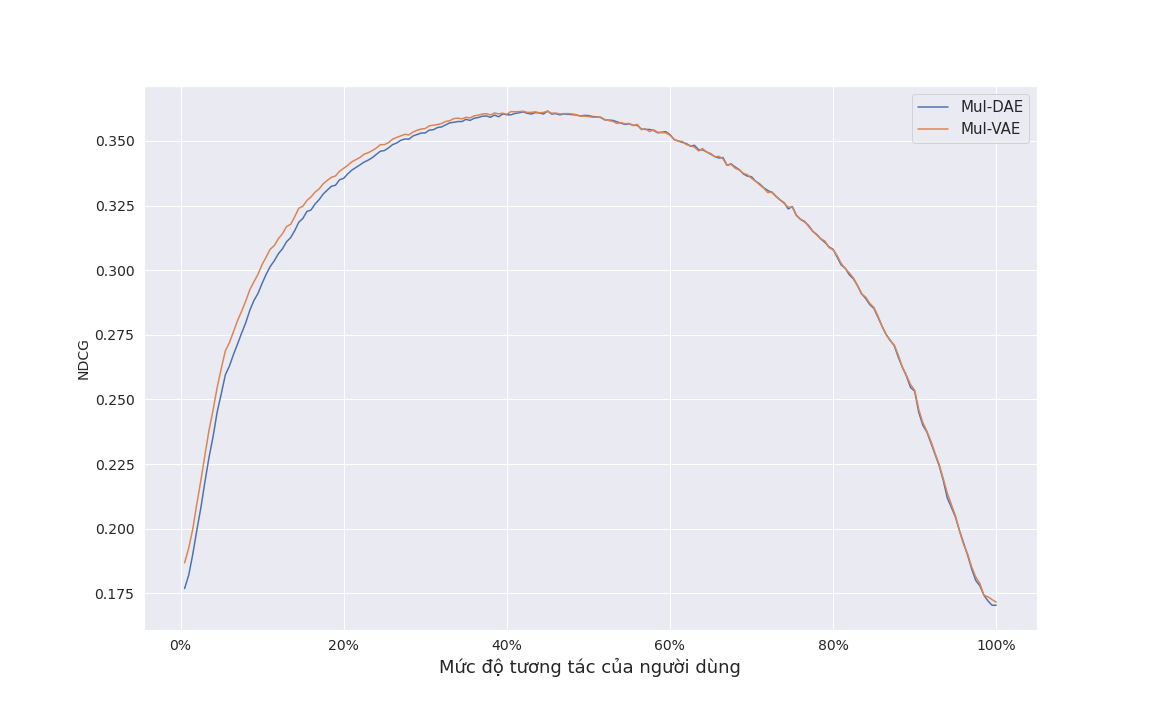
\includegraphics[width=1\textwidth]{vae_dae_msd.png}
        \caption{So sánh Mult-VAE và Mult-DAE ở các mức độ tương tác khác nhau trên tập kiểm tra trên tập Million Song Datasets}
        \label{fig_vae_dae_msd}
    \end{figure}

    Hình \ref{fig_vae_dae_ml} thể hiện giá trị của độ đo NDCG@100 trên tập MovieLens. 
    Với tập dữ liệu này, ta dễ dàng nhận thấy Mult-VAE vượt trội hơn so với Mult-DAE, đặc biệt là khi dữ liệu tương tác người dùng thấp.
    Cụ thể trong khoảng mức độ tương tác của người dùng từ 20\% đến 40\% thì Mult-DAE hoàn toàn bị bỏ xa bởi Mult-VAE.
    Hình \ref{fig_vae_dae_msd} là kết quả thực hiện thí nghiệm trên tập MSD.
    Tập dữ liệu này cũng có xu hướng tương tự như trên tập MovieLens, tuy nhiên sự cách biệt giữa Mult-DAE và Mult-VAE không quá rõ ràng.
    Song, ta vẫn dễ dàng nhận thấy được rằng với mức độ tương tác thấp Mult-VAE vẫn cho kết quả nhỉnh hơn so với Mult-DAE.

    Kết quả thí nghiệm giúp ta đã giúp khẳng định lại được độ hiệu quả của mô hình Mult-VAE được đề xuất trong bài báo \cite{mvae}. 
    Tuy trên tổng quan thì Mult-VAE không quá vượt trội so với Mult-DAE nhưng ở trường hợp dữ liệu tương tác người dùng ở mức độ thấp thì Mult-VAE mang lại kết quả cực kỳ ấn tượng.





\chapter{Kết luận và hướng phát triển}
\label{Chapter5}

\section{Kết luận}
\section{Hướng phát triển}


% Công trình của tác giả (nếu không có thì comment 02 dòng dưới)
% \addcontentsline{toc}{chapter}{Danh mục công trình của tác giả}
% \chapter*{Danh mục công trình của tác giả}
\label{Appendix1}

\begin{enumerate}
\item Tạp chí ABC
\item Tạp chí XYZ
\end{enumerate}

% In tài liệu tham khảo
\addcontentsline{toc}{chapter}{Tài liệu tham khảo}
\printbibliography[title={Tài liệu tham khảo}]
% \printbibliography[heading=subbibliography, title={Tiếng Việt}, keyword=Viet, resetnumbers=true]

% \DeclareNameAlias{sortname}{last-first}
% \DeclareNameAlias{default}{last-first}

% \printbibliography[heading=subbibliography, title={}, notkeyword=Viet, resetnumbers=1] 
% ================================noeets ===================================== %
% CHÚ Ý: phải gán lại resetnumbers=số tài liệu tham khảo tiếng Việt + 1 %
% ===================================================================== %

% % Phần phụ lục
% \appendix

\chapter{PHỤC LỤC}
\label{Appendix1}
\graphicspath{{Appendix/AppendixFigs/}}
\section{Các độ đo đánh giá hệ thống gợi ý}
\label{chap_metrics}
\subsection{NDCG}
\subsection{Recall}
% \chapter{Ngữ pháp tiếng Nôm}
\label{Appendix2}

Đây là phụ lục 2.

\end{document} 